% Judul dokumen
\title{Buku Tugas Akhir ITS}
\author{Musk, Elon Reeve}

% Pengaturan ukuran teks dan bentuk halaman dua sisi
\documentclass[12pt,twoside]{report}

% Pengaturan ukuran halaman dan margin
\usepackage[a4paper,top=30mm,left=30mm,right=20mm,bottom=25mm]{geometry}

% Pengaturan ukuran spasi
\usepackage[singlespacing]{setspace}

% Pengaturan detail pada file PDF
\usepackage[pdfauthor={\@author},bookmarksnumbered,pdfborder={0 0 0}]{hyperref}

% Pengaturan jenis karakter
\usepackage[utf8]{inputenc}

% Pengaturan pewarnaan
\usepackage[table,xcdraw]{xcolor}

% Pengaturan kutipan artikel
\usepackage[style=apa, backend=biber]{biblatex}

% Package lainnya
\usepackage{changepage}
\usepackage{enumitem}
\usepackage{eso-pic}
\usepackage{txfonts} % Font times
\usepackage{etoolbox}
\usepackage{graphicx}
\usepackage{lipsum}
\usepackage{longtable}
\usepackage{tabularx}
\usepackage{wrapfig}
\usepackage{float}

% Definisi untuk "Hati ini sengaja dikosongkan"
\patchcmd{\cleardoublepage}{\hbox{}}{
  \thispagestyle{empty}
  \vspace*{\fill}
  \begin{center}\textit{[Halaman ini sengaja dikosongkan]}\end{center}
  \vfill}{}{}

% Pengaturan penomoran halaman
\usepackage{fancyhdr}
\fancyhf{}
\renewcommand{\headrulewidth}{0pt}
\pagestyle{fancy}
\fancyfoot[LE,RO]{\thepage}
\patchcmd{\chapter}{plain}{fancy}{}{}
\patchcmd{\chapter}{empty}{plain}{}{}

% Command untuk bulan
\newcommand{\MONTH}{%
  \ifcase\the\month
  \or Januari% 1
  \or Februari% 2
  \or Maret% 3
  \or April% 4
  \or Mei% 5
  \or Juni% 6
  \or Juli% 7
  \or Agustus% 8
  \or September% 9
  \or Oktober% 10
  \or November% 11
  \or Desember% 12
  \fi}
\newcommand{\ENGMONTH}{%
  \ifcase\the\month
  \or January% 1
  \or February% 2
  \or March% 3
  \or April% 4
  \or May% 5
  \or June% 6
  \or July% 7
  \or August% 8
  \or September% 9
  \or October% 10
  \or November% 11
  \or December% 12
  \fi}

% Pengaturan format judul bab
\usepackage{titlesec}
\titleformat{\chapter}[display]{\bfseries\Large}{BAB \centering\Roman{chapter}}{0ex}{\vspace{0ex}\centering}
\titleformat{\section}{\bfseries\large}{\MakeUppercase{\thesection}}{1ex}{\vspace{1ex}}
\titleformat{\subsection}{\bfseries\large}{\MakeUppercase{\thesubsection}}{1ex}{}
\titleformat{\subsubsection}{\bfseries\large}{\MakeUppercase{\thesubsubsection}}{1ex}{}
\titlespacing{\chapter}{0ex}{0ex}{4ex}
\titlespacing{\section}{0ex}{1ex}{0ex}
\titlespacing{\subsection}{0ex}{0.5ex}{0ex}
\titlespacing{\subsubsection}{0ex}{0.5ex}{0ex}

% Atur variabel berikut sesuai namanya

% nama
\newcommand{\name}{Adritia Alfiana Merdila}
\newcommand{\authorname}{Merdila, Adritia Alfiana}
\newcommand{\nickname}{Tia}
\newcommand{\advisor}{Ahmad Zaini, S.T., M.Sc}
\newcommand{\coadvisor}{Reza Fuad Rachmadi, S.T., M.T., Ph.D.}
\newcommand{\examinerone}{Dr. Galileo Galilei, S.T., M.Sc}
\newcommand{\examinertwo}{Friedrich Nietzsche, S.T., M.Sc}
\newcommand{\examinerthree}{Alan Turing, ST., MT}
\newcommand{\headofdepartment}{Dr. Supeno Mardi Susiki Nugroho, S.T., M.T.}

% identitas
\newcommand{\nrp}{0721 19 4000 0017}
\newcommand{\advisornip}{19750419 200212 1 003}
\newcommand{\coadvisornip}{19850403 201212 1 001}
\newcommand{\examineronenip}{18560710 194301 1 001}
\newcommand{\examinertwonip}{18560710 194301 1 001}
\newcommand{\examinerthreenip}{18560710 194301 1 001}
\newcommand{\headofdepartmentnip}{19700313199512 1 001}

% judul
\newcommand{\tatitle}{KLASIFIKASI KANTUK BERDASARKAN POLA KEDIPAN MATA dan
POLA BUKAAN MULUT dengan IndRNN}
\newcommand{\engtatitle}{\emph{DROWSINESS CLASSIFICATION BASED ON EYE BLINK PATTERN AND MOUTH OPENING PATTERN USING IndRNN}}

% tempat
\newcommand{\place}{Surabaya}

% jurusan
\newcommand{\studyprogram}{Teknik Komputer}
\newcommand{\engstudyprogram}{Computer Engineering}

% fakultas
\newcommand{\faculty}{Fakultas Teknologi Elektro dan Informatika Cerdas}
\newcommand{\engfaculty}{Faculty of Intelligent Electrical and Informatics Technology}

% singkatan fakultas
\newcommand{\facultyshort}{FTEIC}
\newcommand{\engfacultyshort}{F-ELECTICS}

% departemen
\newcommand{\department}{Teknik Komputer}
\newcommand{\engdepartment}{Computer Engineering}

% kode mata kuliah
\newcommand{\coursecode}{EC224801}


% Tambahkan format tanda hubung yang benar di sini
\hyphenation{
  ro-ket
  me-ngem-bang-kan
  per-hi-tu-ngan
  tek-no-lo-gi
  me-la-ku-kan
  ber-so-si-al-i-sa-si
  pe-num-pang
}

% Menambahkan resource daftar pustaka
\addbibresource{pustaka/pustaka.bib}

% Pengaturan format potongan kode
\usepackage{listings}
\definecolor{comment}{RGB}{0,128,0}
\definecolor{string}{RGB}{255,0,0}
\definecolor{keyword}{RGB}{0,0,255}
\lstdefinestyle{codestyle}{
  commentstyle=\color{comment},
  stringstyle=\color{string},
  keywordstyle=\color{keyword},
  basicstyle=\footnotesize\ttfamily,
  numbers=left,
  numberstyle=\tiny,
  numbersep=5pt,
  frame=lines,
  breaklines=true,
  prebreak=\raisebox{0ex}[0ex][0ex]{\ensuremath{\hookleftarrow}},
  showstringspaces=false,
  upquote=true,
  tabsize=2,
}
\lstset{style=codestyle}

% Isi keseluruhan dokumen
\begin{document}

% Sampul luar Bahasa Indonesia
\newcommand\covercontents{sampul/konten-id.tex}
\AddToShipoutPictureBG*{
  \AtPageLowerLeft{
    % Ubah nilai berikut jika posisi horizontal background tidak sesuai
    \hspace{-3.25mm}

    % Ubah nilai berikut jika posisi vertikal background tidak sesuai
    \raisebox{0mm}{
      
\includegraphics[width=\paperwidth,height=\paperheight]{sampul/gambar/sampul-luar.png}
    }
  }
}

% Menyembunyikan nomor halaman
\thispagestyle{empty}

% Pengaturan margin untuk menyesuaikan konten sampul
\newgeometry{
  top=55mm,
  left=30mm,
  right=20mm,
  bottom=20mm
}

\begin{flushleft}

  % Pemilihan font sans serif
  \sffamily

  % Pemilihan warna font putih
  \color{white}

  % Pemilihan font bold
  \fontseries{bx}
  \selectfont
  \begin{spacing}{1.5}
    \input{\covercontents}
  \end{spacing}

\end{flushleft}

\restoregeometry


% Atur ulang penomoran halaman
\setcounter{page}{1}

% Sampul dalam Bahasa Indonesia
\renewcommand\covercontents{sampul/konten-id.tex}
\AddToShipoutPictureBG*{
  \AtPageLowerLeft{
    % Ubah nilai berikut jika posisi horizontal background tidak sesuai
    \hspace{-4mm}

    % Ubah nilai berikut jika posisi vertikal background tidak sesuai
    \raisebox{0mm}{
      
\includegraphics[width=\paperwidth,height=\paperheight]{sampul/gambar/sampul-luar-tipis.png}
    }
  }
}

% Menyembunyikan nomor halaman
\thispagestyle{empty}

% Pengaturan margin untuk menyesuaikan konten sampul
\newgeometry{
  top=65mm,
  left=30mm,
  right=30mm,
  bottom=20mm
}

\begin{flushleft}

  % Pemilihan font sans serif
  \sffamily

  % Pemilihan font bold
  \fontseries{bx}
  \selectfont
  \begin{spacing}{1.5}
    \input{\covercontents}
  \end{spacing}

\end{flushleft}

\restoregeometry

\clearpage
\cleardoublepage

% Sampul dalam Bahasa Inggris
\renewcommand\covercontents{sampul/konten-en.tex}
\AddToShipoutPictureBG*{
  \AtPageLowerLeft{
    % Ubah nilai berikut jika posisi horizontal background tidak sesuai
    \hspace{-4mm}

    % Ubah nilai berikut jika posisi vertikal background tidak sesuai
    \raisebox{0mm}{
      
\includegraphics[width=\paperwidth,height=\paperheight]{sampul/gambar/sampul-luar-tipis.png}
    }
  }
}

% Menyembunyikan nomor halaman
\thispagestyle{empty}

% Pengaturan margin untuk menyesuaikan konten sampul
\newgeometry{
  top=65mm,
  left=30mm,
  right=30mm,
  bottom=20mm
}

\begin{flushleft}

  % Pemilihan font sans serif
  \sffamily

  % Pemilihan font bold
  \fontseries{bx}
  \selectfont
  \begin{spacing}{1.5}
    \input{\covercontents}
  \end{spacing}

\end{flushleft}

\restoregeometry

\cleardoublepage

% Pengaturan ukuran indentasi paragraf
\setlength{\parindent}{2em}

% Pengaturan ukuran spasi paragraf
\setlength{\parskip}{1ex}

% Lembar pengesahan
\begin{center}
  \large
  \textbf{LEMBAR PENGESAHAN}
\end{center}

% Menyembunyikan nomor halaman
\thispagestyle{empty}

\begin{center}
  \textbf{\tatitle{}}
\end{center}

\begingroup
% Pemilihan font ukuran small
\small

\begin{center}
  \textbf{TUGAS AKHIR}
  \\Diajukan untuk memenuhi salah satu syarat \\
  memperoleh gelar Sarjana Teknik pada \\
  Program Studi S-1 \studyprogram{} \\
  Departemen \department{} \\
  Fakultas \faculty{} \\
  Institut Teknologi Sepuluh Nopember
\end{center}

\begin{center}
  Oleh: \textbf{\name{}}
  \\NRP. \nrp{}
\end{center}

\begin{center}
  Disetujui oleh Tim Penguji Tugas Akhir:
\end{center}

\begingroup
% Menghilangkan padding
\setlength{\tabcolsep}{0pt}

\noindent
\begin{tabularx}{\textwidth}{X l}
  \advisor{}               & (Pembimbing I)                      \\
  NIP: \advisornip{}       &                                     \\
                           &                                     \\
                           &                                     \\
                           & ................................... \\
                           &                                     \\                                                      
  \coadvisor{}             & (Pembimbing II)                     \\
  NIP: \coadvisornip{}     &                                     \\
                           &                                     \\
                           &                                     \\
                           & ................................... \\
                           &                                     \\                                                      
  \examinerone{}.          & (Penguji I)                         \\
  NIP: \examineronenip{}   &                                     \\
                           &                                     \\
                           &                                     \\
                           & ................................... \\
                           &                                     \\                                                      
  \examinertwo{}.          & (Penguji II)                        \\
  NIP: \examinertwonip{}   &                                     \\
                           &                                     \\
                           &                                     \\
                           & ................................... \\                                                     
\end{tabularx}
\endgroup

\begin{center}
  Mengetahui, \\
  Kepala Departemen \department{} \facultyshort{} - ITS\\

  \vspace{8ex}

  \underline{\headofdepartment{}.} \\
  NIP. \headofdepartmentnip{}
\end{center}

\begin{center}
  \textbf{\MakeUppercase{\place{}}\\\MONTH{}, \the\year{}}
\end{center}
\endgroup

\cleardoublepage
\begin{center}
  \large
  \textbf{APPROVAL SHEET}
\end{center}

% Menyembunyikan nomor halaman
\thispagestyle{empty}

\begin{center}
  \textbf{\engtatitle{}}
\end{center}

\begingroup
% Pemilihan font ukuran small
\small

\begin{center}
  \textbf{FINAL PROJECT}
  \\Submitted to fulfill one of the requirements \\
  for obtaining a degree Bachelor of Engineering at \\
  Undergraduate Study Program of \engstudyprogram{} \\
  Department of \engdepartment{} \\
  Faculty of \engfaculty{} \\
  Sepuluh Nopember Institute of Technology
\end{center}

\begin{center}
  By: \textbf{\name{}}
  \\NRP. \nrp{}
\end{center}

\begin{center}
  Approved by Final Project Examiner Team:
\end{center}

\begingroup
% Menghilangkan padding
\setlength{\tabcolsep}{0pt}

\noindent
\begin{tabularx}{\textwidth}{X l}
  \advisor{}               & (Advisor I)                         \\
  NIP: \advisornip{}       &                                     \\
                           &                                     \\
                           &                                     \\
                           & ................................... \\                           
                           &                                     \\                           
  \coadvisor{}             & (Co-Advisor II)                     \\
  NIP: \coadvisornip{}     &                                     \\
                           &                                     \\
                           &                                     \\
                           & ................................... \\                           
                           &                                     \\                           
  \examinerone{}.          & (Examiner I)                        \\
  NIP: \examineronenip{}   &                                     \\
                           &                                     \\
                           &                                     \\
                           & ................................... \\                           
                           &                                     \\                           
  \examinertwo{}.          & (Examiner II)                       \\
  NIP: \examinertwonip{}   &                                     \\
                           &                                     \\
                           &                                     \\
                           & ................................... \\                          
\end{tabularx}
\endgroup


\begin{center}
  Acknowledged, \\
  Head of \engdepartment{} Department \engfacultyshort{} - ITS \\

  \vspace{8ex}

  \underline{\headofdepartment{}.} \\
  NIP. \headofdepartmentnip{}
\end{center}

\begin{center}
  \textbf{\MakeUppercase{\place{}}\\\ENGMONTH{}, \the\year{}}
\end{center}
\endgroup

\cleardoublepage

% Pernyataan keaslian
\begin{center}
  \large
  \textbf{PERNYATAAN ORISINALITAS}
\end{center}

% Menyembunyikan nomor halaman
\thispagestyle{empty}

\vspace{2ex}

% Ubah paragraf-paragraf berikut sesuai dengan yang ingin diisi pada pernyataan keaslian

\noindent Yang bertanda tangan dibawah ini:

\noindent\begin{tabularx}{\textwidth}{l l X}
                         &   &                            \\
  Nama Mahasiswa / NRP   & : & \name{} / \nrp{}           \\
  Departemen             & : & \department{}              \\
  Dosen Pembimbing / NIP & : & \advisor{} / \advisornip{} \\
                         &   &                            \\
\end{tabularx}

Dengan ini menyatakan bahwa Tugas Akhir dengan judul "\tatitle{}" adalah hasil karya sendiri, berfsifat orisinal, dan ditulis dengan mengikuti kaidah penulisan ilmiah.

Bilamana di kemudian hari ditemukan ketidaksesuaian dengan pernyataan ini, maka saya bersedia menerima sanksi sesuai dengan ketentuan yang berlaku di Institut Teknologi Sepuluh Nopember.

\vspace{8ex}

\noindent\begin{tabularx}{\textwidth}{X l}
                     & \place{}, \ENGMONTH{} \the\year{} \\
                     &                                   \\
  Mengetahui         &                                   \\
  Dosen Pembimbing   & Mahasiswa                         \\
                     &                                   \\
                     &                                   \\
                     &                                   \\
                     &                                   \\
                     &                                   \\
  \advisor{}         & \name{}                           \\
  NIP. \advisornip{} & NRP. \nrp{}                       \\
\end{tabularx}

\cleardoublepage
\begin{center}
  \large
  \textbf{STATEMENT OF ORIGINALITY}
\end{center}

% Menyembunyikan nomor halaman
\thispagestyle{empty}

\vspace{2ex}

% Ubah paragraf-paragraf berikut sesuai dengan yang ingin diisi pada pernyataan keaslian

\noindent The undersigned below:

\noindent\begin{tabularx}{\textwidth}{l l X}
                        &   &                            \\
  Name of student / NRP & : & \name{} / \nrp{}           \\
  Department            & : & \engdepartment{}           \\
  Advisor / NIP         & : & \advisor{} / \advisornip{} \\
                        &   &                            \\
\end{tabularx}

Hereby declared that the Final Project with the title of "\engtatitle{}" is the result of my own work, is original, and is written by following the rules of scientific writing.

If in future there is a discrepancy with this statement, then I am willing to accept sanctions in accordance with provisions that apply at Sepuluh Nopember Institute of Technology.

\vspace{8ex}

\noindent\begin{tabularx}{\textwidth}{X l}
                     & \place{}, \ENGMONTH{} \the\year{} \\
                     &                                   \\
  Acknowledged       &                                   \\
  Advisor            & Student                           \\
                     &                                   \\
                     &                                   \\
                     &                                   \\
                     &                                   \\
                     &                                   \\
  \advisor{}         & \name{}                           \\
  NIP. \advisornip{} & NRP. \nrp{}                       \\
\end{tabularx}
\cleardoublepage

% Nomor halaman pembuka dimulai dari sini
\pagenumbering{roman}

% Abstrak Bahasa Indonesia
\begin{center}
  \large\textbf{ABSTRAK}
\end{center}

\addcontentsline{toc}{chapter}{ABSTRAK}

\vspace{2ex}

\begingroup
% Menghilangkan padding
\setlength{\tabcolsep}{0pt}

\noindent
\begin{tabularx}{\textwidth}{l >{\centering}m{2em} X}
  Nama Mahasiswa    & : & \name{}         \\

  Judul Tugas Akhir & : & \tatitle{}      \\

  Pembimbing        & : & 1. \advisor{}   \\
                    &   & 2. \coadvisor{} \\
\end{tabularx}
\endgroup

% Ubah paragraf berikut dengan abstrak dari tugas akhir
Pengemudi merupkan faktor utama terjadinya kecelakaan yang ada di jalanan. Hal tersebut
dilatarbelakangi oleh berbagai faktor salah satunya adalah rasa kantuk.  Gejala dari
rasa kantuk umumnya adalah microsleeps (berkedip dengan durasi lebih dari 500 ms) dan
menguap. Salah satu cara untuk mendeteksi kantuk yaitu dengan metode non-intrusif
menggunakan visi komputer dengan menerapkan algoritma \emph{Deep Learning}. \emph{Recurrent Neural Network} merupakan
salah satu jenis \emph{Deep Learning} yang melibatkan masukan berurutan karena memiliki memori
untuk menyimpan \emph{state}. IndRNN merupakan pengembangan dari RNN namun pemrosesan setiap
neuron pada suatu layer tidak bergantung dengan layer lain. Melalui penelitian ini
model klasifikasi kantuk akan dibuat dengan menggunakan parameter kedipan mata dan
pola bukaan mulut dengan menggunakan IndRNN. Penelitian ini mengambil data berupa
video dari database UTA-RLDD. Data tersebut kemudian diproses sehingga
didapatkan nilai \emph{Eye Aspect Ratio} (EAR) dan \emph{Mouth Aspect Ratio} (MAR) pada
setiap frame. EAR dan MAR tersebut nantinya akan digunakan sebagai masukan model
klasifikasi pada IndRNN yang menghasilkan output berupa 3 kelas yang mengacu pada skala
kantuk Karolinska. Kelas tersebut diantaranya : Kelas pertama (Waspada) yaitu
terdiri dari label kelas KSS 1 sampai 5, Kelas kedua (Waspada Rendah) yaitu terdiri dari
label kelas KSS 6 dan 7, Kelas ketiga (Mengantuk) yaitu terdiri dari label kelas
KSS 8 dan 9. Berdasarkan penelitian yang telah dilakukan, model klasifikasi kantuk yang 
paling efektif adalah model IndRNN dengan data teraugmentasi. Model tersebut memiliki 
nilai akurasi sebesar 0,6943 dan niali validasi sebesar 0,52.

% Ubah kata-kata berikut dengan kata kunci dari tugas akhir
Kata Kunci: IndRNN, Kantuk, Visi Komputer.

\cleardoublepage

% Abstrak Bahasa Inggris
\begin{center}
  \large\textbf{ABSTRACT}
\end{center}

\addcontentsline{toc}{chapter}{ABSTRACT}

\vspace{2ex}

\begingroup
% Menghilangkan padding
\setlength{\tabcolsep}{0pt}

\noindent
\begin{tabularx}{\textwidth}{l >{\centering}m{3em} X}
  \emph{Name}     & : & \name{}         \\

  \emph{Title}    & : & \engtatitle{}   \\

  \emph{Advisors} & : & 1. \advisor{}   \\
                  &   & 2. \coadvisor{} \\
\end{tabularx}
\endgroup

% Ubah paragraf berikut dengan abstrak dari tugas akhir dalam Bahasa Inggris
\emph{The driver is the main factor in the occurrence of accidents on the road. This is motivated by
various factors one of which is drowsiness. Common symptoms of drowsiness are microsleeps
(blinks longer than 500 ms) and yawning. One way to detect drowsiness is by using a non-intrusive
method using computer vision by applying the Deep Learning algorithm. RNN is a type of Deep
Learning that involves sequential input because it has memory to store state. IndRNN is a 
development of RNN but the processing of each neuron in a layer is independent of other layers.
Through this research a drowsiness classification model will be created using the parameters
of eye blink and mouth opening pattern using IndRNN. This study retrieved data in the form of
videos from the DROZY and UTA-RLDD databases. The data is then processed to obtain the Eye
Aspect Ratio (EAR) and Mouth Aspect Ratio (MAR) values for each frame. The EAR and MAR will
later be used as input for the classification model in IndRNN which produces output in the
form of 3 classes that refer to the Karolinska sleepiness scale. These classes include: First
class (Alert) which consists of class labels KSS 1 to 5, Second class (Low Vigilant) which
consists of class labels KSS 6 and 7, Third class (Drowsy) which consists of class labels
KSS 8 and 9. Based on the conducted research, the most effective drowsiness classification model 
is the IndRNN model with augmented data. It achieved an accuracy score of 0.6943 and a validation 
score of 0.52.}

% Ubah kata-kata berikut dengan kata kunci dari tugas akhir dalam Bahasa Inggris
\emph{Keywords}: \emph{Computer Vision, Drowsiness, IndRNN}.

\cleardoublepage

% Kata pengantar
\begin{center}
  \Large
  \textbf{KATA PENGANTAR}
\end{center}

\addcontentsline{toc}{chapter}{KATA PENGANTAR}

\vspace{2ex}

% Ubah paragraf-paragraf berikut dengan isi dari kata pengantar

Puji dan syukur atas kehadirat Allah SWT yang telah
melimpahkan rahmat, nikmat, serta hidayah-Nya sehingga skripsi yang berjudul
\textbf{\tatitle{}} dapat diselesaikan dengan baik.

Penelitian ini disusun dalam rangka memenuhi salah satu syarat
kelulusan Program Studi S-1 Teknik Komputer Departemen Teknik
Komputer Fakultas Teknologi Elektro dan Informatika Cerdas
Institut Teknologi Sepuluh Nopember. Tugas akhir ini mustahil
diselesaikan tanpa adanya dukungan dan bimbingan dari berbagai
pihak. Oleh karena itu, penulis mengucapkan terima kasih kepada:

\begin{enumerate}[nolistsep]

  \item Bapak \advisor{} selaku dosen pembimbing I yang telah banyak memberikan semangat, masukan,
        serta arahan kepada penulis mengenai penelitian dan penulisan buku Tugas Akhir.

  \item Bapak \coadvisor{} selaku dosen pembimbing II yang telah banyak
        memberikan masukan serra arahan pada pengerjaan penelitian dan penulisan buku Tugas Akhir.

  \item Ibu, Ayah dan Saudara yang selalu mendoakan dan mendukung penulis secara emosional maupun finansial.

  \item Teman-teman tercinta yang selalu ada untuk penulis dan senantiasa memberikan semangat kepada penulis.

  \item Bapak dan Ibu Dosen Teknik Komputer ITS untuk segala ilmu dan motivasi yang telah diberikan selama perkuliahan.

  \item Bapak dan Ibu staff karyawan Teknik Komputer ITS untuk segala usahanya untuk menciptakan lingkungan perkuliahan yang nyaman.

\end{enumerate}

Proposal ini jauh dari kata sempurna. Oleh karena itu penulis
mengharapkan kritik dan saran yang dapat digunakan untuk meningkatkan dan mengoreksi
penelitian ini. Akhir kata, semoga penelitian yang telah dibuat dapat bermanfaat
dan dapat diterima dengan baik oleh banyak pihak.

\begin{flushright}
  \begin{tabular}[b]{c}
    \place{}, \MONTH{} \the\year{} \\
    \\
    \\
    \\
    \\
    \name{}
  \end{tabular}
\end{flushright}

\cleardoublepage

% Daftar isi
\renewcommand*\contentsname{DAFTAR ISI}
\addcontentsline{toc}{chapter}{\contentsname}
\tableofcontents
\cleardoublepage

% Daftar gambar
\renewcommand*\listfigurename{DAFTAR GAMBAR}
\addcontentsline{toc}{chapter}{\listfigurename}
\listoffigures
\cleardoublepage

% Daftar tabel
\renewcommand*\listtablename{DAFTAR TABEL}
\addcontentsline{toc}{chapter}{\listtablename}
\listoftables
\cleardoublepage

% Nomor halaman isi dimulai dari sini
\pagenumbering{arabic}

% Bab 1 pendahuluan
\chapter{PENDAHULUAN}
\label{chap:pendahuluan}

% Ubah bagian-bagian berikut dengan isi dari pendahuluan

\section{Latar Belakang}
\label{sec:latarbelakang}

Seorang pengemudi harus bisa bertanggung jawab terhadap
keselamatan pribadinya, penumpang ataupun barang yang dibawa.
Oleh karena itu, pengemudi perlu fokus hingga sampai ke tempat
tujuan dikarenakan mengemudi ialah kegiatan yang monoton, dengan
tugas yang berulang-ulang dan memerlukan perhatian berkelanjutan
\parencite{1}. Mengantuk, didefinisikan sebagai keadaan kantuk
ketika seseorang perlu istirahat. Mengantuk dapat menyebabkan gejala yang
berdampak besar terhadap kinerja tugas seperti: waktu respons
yang melambat, kurangnya kesadaran intermiten, atau \emph{microsleeps}
(berkedip dengan durasi lebih dari 500 ms) \parencite{2}. Ciri
lain dari orang yang mengantuk adalah sering menguap pada jangka
waktu tertentu \parencite{3}. Saat mengemudi, gejala-gejala ini
sangat berbahaya karena secara signifikan meningkatkan kemungkinan
terlewatnya rambu-rambu jalan atau pintu keluar, hanyut ke jalur
lain atau bahkan kecelakaan \parencite{4}.

Mendeteksi kantuk merupakan salah satu cara untuk menghindari
dampak negatif dari rasa kantuk itu sendiri. Beberapa cara dapat
digunakan untuk mendeteksi rasa kantuk contohnya dengan metode
intrusif dimana pendeteksian rasa kantuk dilakukan dengan memanfaatkan
bantuan alat EKG (\emph{Electrocardiogram}) dan EEG (\emph{Electroencephalogram}).
Selain itu ada juga metode non-intrusif yaitu dengan melakukan ekstraksi pada
fitur wajah dengan menggunakan algoritma tertentu.

Algoritma \emph{Deep Learning} dicirikan oleh penggunaan jaringan saraf
yang dibangun dari jumlah lapisan yang besar \parencite{5}, jaringan
saraf tersebut memiliki kemampuan untuk mengotomatisasi proses ekstraksi
fitur \parencite{6}. Dalam deep learning, algoritmanya dapat mempelajari
representasi data yang lebih abstrak dan kompleks secara bertahap melalui
lapisan-lapisan yang ada dalam dalam jaringan saraf. Setiap lapisan dalam
jaringan saraf tiruan ini bertanggung jawab untuk memproses informasi secara
bertingkat, menggabungkan dan mentransformasikan data pada setiap langkahnya.

\emph{Recurrent neural networks} (RNN) merupakan salah satu jenis
dari algoritma \emph{Deep Learning} yang banyak digunakan untuk tugas
dengan input berurutan, seperti ucapan dan bahasa. Kinerja RNN lebih baik
untuk data input berurutan karena mempunyai memori yang bisa
dipergunakan untuk menyimpan state \parencite{18}. Pada tahun 2018,
Shuali Li et al. mengatakan \emph{Independently Recurrent Neural Network}
(IndRNN) yakni variasi \emph{deep learning} RNN. Bersumberkan pada
penelitian Shuali Li et al. (2018), IndRNN ini 10 kali lebih cepat
serta sedikit lebih akurat dari implementasi \emph{deep learning Long Short-Term Memory}
(LSTM) yang selalu dipergunakan \parencite{8}.

Dengan akurasi pendeteksian kantuk yang baik maka berbagai masalah yang timbul dari 
rasa kantuk saat berkendara tersebut dapat dihindari. Sebuah model untuk menentukan 
tingkat kantuk seseorang diperlukan karena dapat digunakan sebagai bahan penelitian 
yang berkaitan.

\newpage
\section{Rumusan Masalah}
\label{sec:permasalahan}

Bersumberkan latar belakang pada sub-bab 1.1, penggunaan EKG dan
EEG dirasa tidak tepat untuk penggunaan sehari-hari karena memerlukan
bantuan ahli untuk menggunakan alat-alat tersebut dengan tepat.
Pengendara akan merasa kesulitan saat harus menggunakan alat-alat
penunjang sebelum mengemudikan kendaraannya. Oleh karena itu
diperlukan metode non intrusif, dimana sistem akan mendeteksi
rasa kantuk dengan mengimplementasikan \emph{deep learning} untuk
mengklasifikasikan tingkat kantuk pengemudi.

\section{Tujuan}
\label{sec:Tujuan}

Tujuan dari penelitian ini adalah membangun sistem klasifikasi
kantuk menggunakan algoritma IdnRNN dengan parameter pola kedipan
mata serta pola bukaan mulut yang dapat mengklasifikasikan kantuk
menjadi 3 kelas berbeda yaitu waspada, kewaspadaan rendah, mengantuk.

\section{Batasan Masalah}
\label{sec:batasanmasalah}

Batasan-batasan dari proyek penelitian ini adalah:

\begin{enumerate}[nolistsep]

      \item Data yang digunakan pada penelitian ini adalah video
            dari \emph{The University of Texas at Arlington Real-Life Drowsiness Dataset (UTA-RLDD)}.

      \item Model akan mendeteksi kantuk berdasarkan pola kedipan
            mata serta pola bukaan mulut.

      \item Model hanya akan memproses video masukan dengan durasi
            tercepat 9 menit dan dengan jumlah \emph{frame per second}
            sebesar 30.

      \item Model akan mengklasifikasikan video dalam 3 kelas kantuk
            yaitu kelas 1 (Waspada), kelas 2 (Kewaspadaan Rendah),
            dan kelas 3 (Mengantuk).

\end{enumerate}

\section{Manfaat}

% Ubah paragraf berikut sesuai dengan tujuan penelitian dari tugas akhir
Manfaat dari penelitian ini diantaranya :
\subsection{Bagi Penulis}
Sebagai sarana implementasi ilmu yang telah didapatkan pada masa
perkuliahan khususnya mengenai \emph{computer vision} dan \emph{deep learning}, melatih penulis untuk bisa
berpikir secara logis, sistematis, dan kritis dalam pemecahan masalah sehingga dapat
memecahkan permasalahan di kehidupan nyata seperti klasifikasi kantuk pada pengemudi.
\subsection{Bagi Institusi}
Sebagai pedoman serta inspirasi bagi penelitian lain yang
berfokus pada pemecahan masalah klasifikasi kantuk menggunakan \emph{deep learning} khususnya dengan
metode IndRNN.
\subsection{Bagi Masyarakat}
Harapannya solusi yang dibuat pada penelitian ini bisa dilaksanakan serta digunakan
menjadi produk nyata yang manfaatnya bisa dirasakan langsung oleh masyarakat sehingga dapat
mengurangi dampak negatif dari rasa kantuk itu sendiri.

\cleardoublepage

% Bab 2 tinjauan pustaka
\chapter{TINJAUAN PUSTAKA}
\label{chap:tinjauanpustaka}

% Ubah bagian-bagian berikut dengan isi dari tinjauan pustaka

\section{Hasil penelitian terdahulu}

Berdasarkan tinjauan literatur yang mencakup beberapa penelitian mengenai pengembangan
sistem deteksi kantuk secara non intrusif menggunakan pengolahan citra atau \emph{machine learning},
penelitian sebelumnya menjadi relevan dan penting untuk dikaji. Mengacu pada referensi penelitian
terdahulu akan membantu mencegah plagiarisme atau duplikasi hasil penelitian. Hal ini
bertujuan untuk memberikan kontribusi bagi penulis dan memastikan bahwa penelitian
mengenai tema ini dapat terus berkembang. Berikut adalah beberapa ulasan tentang
penelitian terdahulu yang pernah dilakukan.

\subsection{Pengembangan Sistem Deteksi Kantuk Menggunakan Pengklasifikasi \emph{Random Forest} pada Sinyal Elektrokardiogram}
Pada penelitian ini Nuryani Nuryani, Khoirun Nisak, Artono Dwijo Sutomo mengembangkan   sistem   deteksi   kantuk
memakai   sinyal elektrokardiogram  (EKG)  dan \emph{Random  Forest}. Sistem  deteksi kantuk   dilatih   memakai suatu
rekaman   EKG   dari database DROZY yang dilengkapi \emph{Karolinska Sleepiness Scale}(KSS). Fitur masukan  sistem  diekstraksi
bersumberkan pada  metode ranah waktu serta ranah frekuensi \parencite{9}.

\subsection{Deteksi Kantuk Berdasarkan Pola Bukaan Mulut Menggunakan Metode 1D CNN}
Pada penelitian ini Victorio Valendion melakukan riset tentang deteksi kantuk memakai landmark bagian mulut melalui
memperhitungkan pola dari terbuka serta tertutup-nya mulut. Nilai dari rasio bukaan mulut dihitung selanjutnya
semua data nya disimpan ke dalam suatu file csv yang kemudian akan dilakukan proses pelatihan untuk mesin
supaya dapat mendeteksi kantuk dengan arsitektur 1D CNN \parencite{10}.

\subsection{Klasifikasi Skala Kantuk Karolinska Berdasarkan Nilai \emph{Eye Aspect Ratio} Menggunakan \emph{Deep Learning}}
Pada penelitian ini Annida Miftakhul Farodisa melakukan riset tentang deteksi kantuk menggunakan metode non-intrusif
dengan memanfaatkan kamera (fitur wajah) dan \emph{deep learning}. Penulis membuat model klasifikasi Skala Kantuk Karolinska
(SKK) berdasarkan nilai \emph{Eye Aspect Ratio}. Penelitian ini menggunakan video \emph{near-infrared} NIR pada dataset DROZY yang berisi video
subjek saat menjalani pengujian kewaspadaan psikomotorik yang mengisi kuesioner Skala Kantuk Karolinska (SKK) sebelum
memulai pengujian. Dilakukan ekstraksi nilai EAR untuk setiap subjek pada setiap frame di setiap video sehingga
membentuk pola EAR dan dilabeli dengan SKK yang dikelompokkan menjadi empat kelas \parencite{11}.

\subsection{Deteksi Kantuk Pada Pengendara Roda Empat Melalui Citra Wajah Menggunakan Metode \emph{Facial Landmark}}
Pada penelitian ini Muhammad Akbar Maulana melakukan riset tentang deteksi kantuk pada pengendara roda empat melalui
citra wajah memakai metode facial landmark. Membuat suatu sistem yang bisa memperingatkan pengemudi secara otomatis
jika pengemudi memperlihatkan gejala mengantuk ketika mengendarai kendaraan akhirnya diharapkan bisa mengurangi
resiko kecelakaan yang bisa terjadi kepada pengendara tersebut. Guna menetapkan pengendara mengantuk ataupun tidak
sistem ini menggunakan algoritma \emph{regression trees} dengan mengambil 2 parameter (\emph{eye blink and Mouth detector}) \parencite{12}.

\section{\emph{Library} Dlib}

Dlib merupakan library open source populer dalam bidang computer vision dan
machine learning. Dlib menyediakan berbagai algoritma dan fungsi yang berguna untuk
berbagai tugas seperti deteksi objek, pengenalan wajah, estimasi pose, deteksi landmark,
pengolahan citra, dan lainnya. Dlib dapat berjalan di berbagai platform seperti Windows,
macOS, Linux, dan Android \parencite{14}. Algoritma deteksi wajah Dlib menggunakan
metode Histogram of Oriented Gradients (HOG) yang dikombinasikan dengan Support Vector
Machines (SVM) untuk menghasilkan deteksi yang akurat. Dlib memiliki kemampuan untuk mendeteksi landmark pada wajah,
yaitu titik-titik penting seperti mata, hidung, dan mulut. Deteksi landmark ini berguna
dalam berbagai aplikasi seperti estimasi pose wajah, analisis ekspresi wajah, dan
penerapan makeup virtual.

\section{\emph{Facial Landmark}}
\emph{Facial Landmark} merupakan ekstraksi titik-titik pada wajah yang tersebar menggunakan detektor wajah \parencite{15}.  Pendeteksi
\emph{facial landmark} diaplikasikan ke \emph{input frames} untuk mendeteksi fitur wajah dengan menggunakan \emph{library} dlib yang
menggunakan \emph{Histogram Oriented Gradients} (HOG) untuk pendeteksian wajah dan \emph{Linear Support Vector Machine} (SVM)
sebagai \emph{classifier} dalam prosedur pengenalan landmark wajah \parencite{16}. Terdapat 68 titik yang merepresentasikan wajah,
titik koordinat tersebut merepresentasikan fitur sesuai dengan gambar \ref{fig:wajah} dan dengan keterangan tiap koordinat pada
tabel \ref{tb:LandmarkWajah}.

\begin{figure} [ht] \centering
  % Nama dari file gambar yang diinputkan
  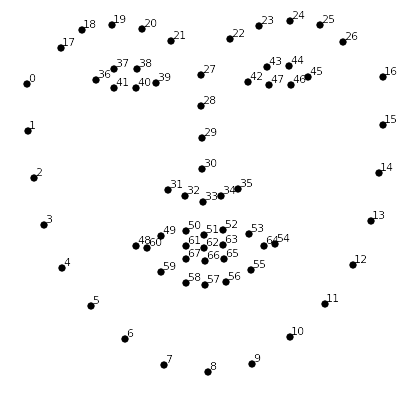
\includegraphics[scale=0.5]{gambar/wajah.png}
  % Keterangan gambar yang diinputkan
  \caption{Landmark wajah manusia \parencite{16}}
  % Label referensi dari gambar yang diinputkan
  \label{fig:wajah}
\end{figure}

\newpage
\begin{longtable}{|c|c|c|}
  \caption{Koordinat landmark wajah}
  \label{tb:LandmarkWajah}                                \\
  \hline
  \rowcolor[HTML]{C0C0C0}
  \textbf{No} & \textbf{Fitur} & \textbf{Koordinat Fitur} \\
  \hline

  % Gunakan \G untuk mengisi sel dan \w untuk mengosongkan sel
  1           & Dagu           & 0-16                     \\
  

  2           & Alis Kanan     & 17-21                    \\
  

  3           & Alis Kiri      & 22-26                    \\
  

  4           & Hidung         & 27-35                    \\
  

  5           & Mata Kanan     & 36-41                    \\
  

  6           & Mata Kiri      & 42-47                    \\
  

  7           & Mulut          & 48-60                    \\
  

  8           & Bibir          & 61-67                    \\
  \hline
\end{longtable}

\subsection{\emph{Eye Aspect Ratio} (EAR)}
EAR merupakan salah satu metode yang dapat digunakan untuk bisa menghitung jarak antara kelopak mata atas serta
kelopak mata bawah bersumberkan titik geometri wajah pada mata. Metode EAR ini selalu dipergunakan untuk menghitung
pola bukaan mata individual setiap menitnya. Perhitungan EAR ini dihitung bersumberkan pada koordinat mata kiri serta
kanan yang ada dalam landmark wajah. EAR pada landmark wajah bisa diilustrasikan denggan gambar \ref{fig:mata} :

\begin{figure} [ht] \centering
  % Nama dari file gambar yang diinputkan
  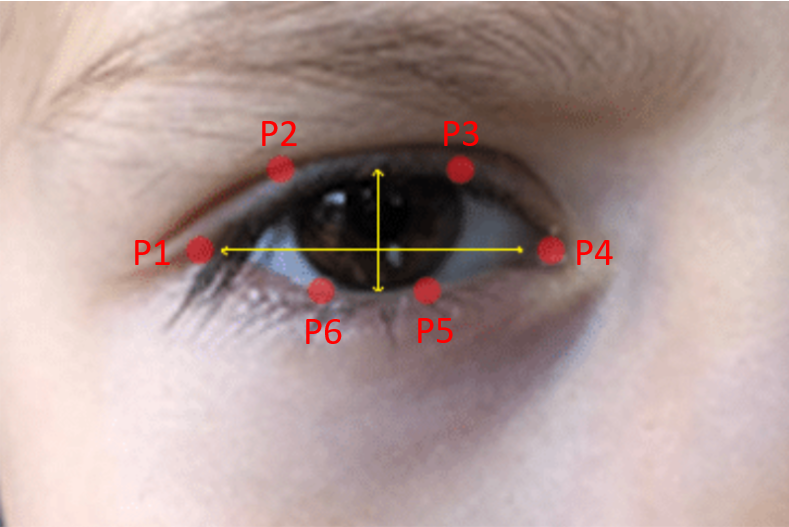
\includegraphics[scale=0.35]{gambar/mata.png}
  % Keterangan gambar yang diinputkan
  \caption{enam titik landmark pada mata \parencite{20}}
  % Label referensi dari gambar yang diinputkan
  \label{fig:mata}
\end{figure}

Nilai EAR didapati dari menghitung jarak antara kelopak mata yang didapatkan melalui mengambil titik tepat ditengah
kelopak mata atas serta kelopak mata bawah. Rumus tersebut dapat dituliskan sesuai rumus \ref{eq:EAR}:

% Contoh pembuatan persamaan
\begin{equation}
  % Label referensi dari persamaan yang dibuat
  \label{eq:EAR}
  % Baris kode persamaan yang dibuat
  EAR = \frac{\left \| P2-P6 \right \| + \left \| P3-P5 \right \|}{2 \left \| P1-P4 \right \|}
\end{equation}

Ketika mata berkedip, dibutuhkan 100 - 400 ms untuk menutup. Perihal ini diperkuat oleh penelitian yang diselengarakan
oleh Caffier et al., yang menyatakan bahwasanya mata tertutup membutuhkan sekitar 200 ms. Sedangkan saat mengantuk,
mata membutuhkan lebih dari 500 ms untuk menutup. Itu perkiraan mata tertutup dimulai saat mata mulai menutup sampai
sepenuhnya tertutup \parencite{17}.

\subsection{\emph{Mouth Aspect Ratio} (MAR)}
MAR ialah salah satu metode yang dapat dipergunakan untuk dapat menghitung jarak antara bibir atas dan bibir bawah
bersumberkan titik geometri wajah pada mulut. Metode MAR ini selalu dipakai guna menghitung bukaan mulut seseorang \parencite{12}.
MAR pada landmark wajah bisa diilustrasikan dengan gambar \ref{fig:mulut} :

\begin{figure} [ht] \centering
  % Nama dari file gambar yang diinputkan
  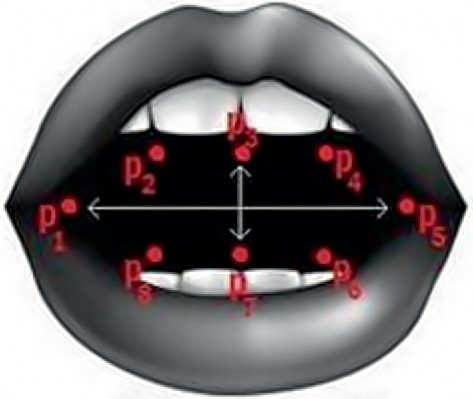
\includegraphics[scale=0.4]{gambar/mulut.png}
  % Keterangan gambar yang diinputkan
  \caption{Enam titik landmark pada mulut \parencite{21}}
  % Label referensi dari gambar yang diinputkan
  \label{fig:mulut}
\end{figure}

Perhitungan nilai MAR sama dengan perhitungan nilai EAR yaitu dengan menghitung jarak antara bibir yang diambil dengan
mengambil titik tepat ditengah bibir atas dan bibir bawah. Rumus tersebut dapat dituliskan menjadi rumus \ref{eq:MAR}:

\begin{equation}
  % Label referensi dari persamaan yang dibuat
  \label{eq:MAR}
  % Baris kode persamaan yang dibuat
  MAR = \frac{\left \| P2-P8 \right \| + \left \| P3-P7 \right \| + \left \| P4-P6 \right \|}{3 \left \| P1-P5 \right \|}
\end{equation}

\section{Skala Kantuk Karolinska(SKK)}
Skala Kantuk Karolinska menjadi alat yang paling banyak digunakan untuk perhitungan kewaspadaan dalam investigasi
kronobiologis dan tidur. SKK ditemukan menjadi pengukur kantuk yang andal dan sensitif (Gillberg et al., 1994), dan
itu divalidasi oleh beberapa pengukuran fisiologis yang berbeda (Kaida et al., 2006; Marzano et al., 2007; Filtness
et al., 2021). Untuk mendeteksi transisi antara terjaga dan tidur dapat diukur menggunakan indeks fisiologis
sederhana yang diambil dan ditentukan dari rekaman \emph{electroencephalogram} (EEG). Nilai pada SKK berkisar antara 1
(amat sangat terjaga) hingga 9 (sangat mengantuk, berusaha lebih untuk terjaga) \parencite{19}. Hal tersebut dapat
digambarkan menjadi seperti tabel \ref{tbl:Skala}:

\begin{longtable}{|c|c|}
  \caption{Skala Kantuk Karolinska \parencite{19}}
  \label{tb:Skala}                                                \\
  \hline
  \rowcolor[HTML]{C0C0C0}
  \textbf{Skala} & \textbf{Tingkat Kantuk / Keterjagaan}          \\
  \hline

  % Gunakan \G untuk mengisi sel dan \w untuk mengosongkan sel
  1              & Amat Sangat Terjaga                            \\
  

  2              & Sangat Terjaga                                 \\
  

  3              & Terjaga                                        \\
  

  4              & Sedikit Terjaga                                \\
  

  5              & Tidak Terjaga namun Tidak ada tanda Mengantuk  \\
  

  6              & Sedikit Mengantuk                              \\
  

  7              & Mengantuk, sedikit usaha untuk Terjaga         \\
  

  8              & Mengantuk, perlu usaha untuk Terjaga           \\
  \hline

  \rowcolor[HTML]{C0C0C0}
  \textbf{Skala} & \textbf{Tingkat Kantuk / Keterjagaan}          \\
  \hline
  9              & Sangat Mengantuk, berusaha lebih untuk Terjaga \\
  \hline
\end{longtable}
\section{Interpolasi Data}

Interpolasi dilakukan untuk mengisi atau memperkirakan nilai yang hilang atau
tidak tersedia dalam dataset dengan menggunakan teknik-teknik yang sesuai. Dalam
beberapa kasus, dataset yang dikumpulkan mungkin tidak lengkap atau terdapat
kehilangan data pada beberapa fitur. \parencite{24}. Beberapa teknik interpolasi
data yang umum digunakan dalam machine learning meliputi:

\begin{enumerate}[nolistsep]
  \item Interpolasi Linear: Teknik ini melibatkan estimasi nilai yang hilang berdasarkan
        hubungan linear antara titik data yang diketahui. Interpolasi linear digunakan
        jika data memiliki hubungan linier yang jelas antara fitur-fitur yang terlibat.

  \item Interpolasi Nearest Neighbor: Metode ini mengisi nilai yang hilang dengan
        menggunakan nilai terdekat dari data terdekat dalam dataset.
        data terdekat dapat ditentukan berdasarkan jarak Euclidean atau metode lainnya.

  \item Interpolasi Polinomial: Metode ini melibatkan pendekatan fungsi polinomial
        untuk mengisi nilai yang hilang. Polinom dapat disesuaikan dengan data yang tersedia
        untuk memperkirakan nilai yang hilang.

  \item Interpolasi Kriging: Teknik ini merupakan metode stokastik yang menggunakan
        model spasial untuk memprediksi nilai yang hilang berdasarkan korelasi spasial antara
        data yang diketahui.

  \item Interpolasi Regresi: Pendekatan ini melibatkan penggunaan model regresi untuk
        memperkirakan nilai yang hilang berdasarkan hubungan antara atribut-atribut yang
        tersedia.
\end{enumerate}

\section{Normalisasi}

Normalisasi dadalah proses mengubah skala nilai dari fitur-fitur dalam dataset
agar memiliki distribusi data yang seragam atau terstandarisasi. Tujuan normalisasi
adalah untuk memastikan bahwa fitur-fitur dengan skala yang berbeda memiliki pengaruh
yang sebanding terhadap proses pembelajaran algoritma \parencite{25}. Beberapa metode
normalisasi umum digunakan adalah sebagai berikut:

\begin{enumerate}[nolistsep]
  \item Min-Max Scaling: Metode ini mentransformasikan setiap nilai fitur menjadi r
        entang yang ditentukan, biasanya antara 0 dan 1. Rumus umum untuk melakukan
        normalisasi Min-Max Scaling adalah sebagai berikut:
        \begin{equation}
          % Label referensi dari persamaan yang dibuat
          \label{eq:MinMax}
          % Baris kode persamaan yang dibuat
          X' = \frac{X - Xmin}{Xmax - Xmin}
        \end{equation}
        Pada rumus \ref{eq:MinMax} X merupakan nilai asli, X' merupakan nilai yang telah
        dinormalisasi, Xmin adalah nilai minimum yang ada pada dataset, dan Xmax adalah nilai
        maksimum yang ada pada dataset.

  \item Z-Score Scaling: Metode ini mengubah nilai fitur menjadi distribusi standar
        dengan mean (rata-rata) 0 dan standard deviation (deviasi standar) 1. Rumus umum
        untuk melakukan normalisasi Z-Score Scaling adalah sebagai berikut:
        \begin{equation}
          % Label referensi dari persamaan yang dibuat
          \label{eq:StandardScaler}
          % Baris kode persamaan yang dibuat
          X' = \frac{X - mean}{stdDev}
        \end{equation}
        Pada rumus \ref{eq:StandardScaler} X merupakan nilai asli, X' merupakan nilai yang telah
        dinormalisasi, mean merupakan nilai rata-rata fitur yang ada pada dataset, dan stdDev
        merupakan nilai standar deviasi dari fitur yang ada pada dataset.
\end{enumerate}

\section{Augmentasi Data}
Augmentasi data merupakan teknik yang digunakan untuk memperbanyak jumlah data dengan
cara memodifikasi data yang telah ada sehingga dapat meningkatkan variasi dalam dataset
pelatihan tanpa harus mengumpulkan lebih banyak data aktual. Jumlah data yang sedikit menjadi alasan dilakukannya
teknik augmentasi data. Data baru yang diperoleh dari proses augmentasi data dapat digunakan
sebagai masukan bagi model \emph{machine learning}. Augmentasi data dapat meningkatkan
performa model dapat dan digunakan untuk mencegah overfitting serta meningkatkan kemampuan
model untuk menggeneralisasi dengan lebih baik. Teknik umum dalam melakukan augmentasi data
diantaranya pemutaran dan pemotongan, pergeseran, perubahan skala, pencerahan dan Kontras,
pembalikan, perubahan warna. \parencite{30}

\section{\emph{Deep Learning}}
\emph{Deep Learning} memungkinkan model komputasi yang memuat atas sejumlah lapisan pemrosesan guna memahami representasi data
melalui sejumlah tingkatan abstraksi. Metode-metode ini sudah meningkatkan \emph{state-of-the-art} dalam pengenalan suara,
pengenalan objek visual, deteksi objek serta banyak domain lainnya secara dramatis. \emph{Deep Learning} mendapati struktur
rumit dalam kumpulan data besar yang memakai algoritma backpropagation guna memperlihatkan bagaimana mesin perlu merubah
parameter internalnya yang dipakai guna memperhitungkan representasi di setiap lapisan dari representasi di lapisan
sebelumnya. \emph{Deep Convolutional Network} mendapatkan terobosan dalam pemrosesan gambar, video, ucapan, serta audio,
sementara \emph{Recurrent Neural Network} menyoroti data berurutan berupa teks serta ucapan \parencite{18}.

\section{\emph{Recurrent Neural Network} (RNN)}

Untuk tugas yang melibatkan input berurutan, seperti ucapan dan bahasa, seringkali lebih baik untuk menggunakan RNN.
RNN mempunyai memori yang bisa dipergunakan untuk menyimpan state, memori ini memungkinkan RNN untuk memiliki pemahaman
tentang konteks sebelumnya saat memproses langkah berikutnya. RNN memproses urutan input satu elemen pada setiap waktu,
mempertahankan di unit tersembunyi mereka sebuah \emph{state vektor} yang secara implisit berisi informasi tentang sejarah semua
elemen masa lalu dari urutannya yang bisa diilustrasikan dengan gambar \ref{fig:rnn}.

\newpage
\begin{figure} [ht] \centering
  % Nama dari file gambar yang diinputkan
  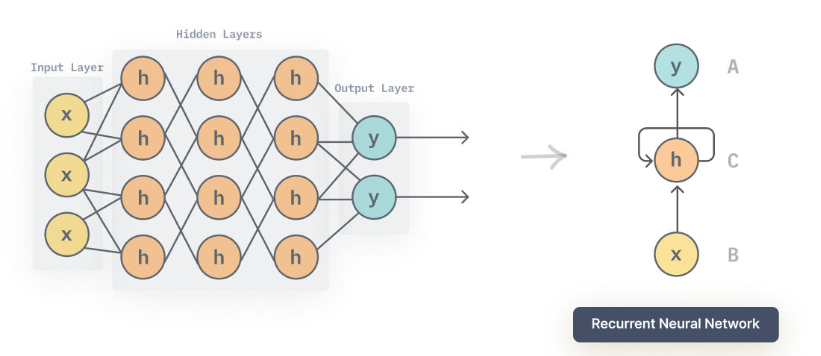
\includegraphics[scale=0.55]{gambar/rnn.png}
  % Keterangan gambar yang diinputkan
  \caption{Ilustrasi RNN \parencite{18}}
  % Label referensi dari gambar yang diinputkan
  \label{fig:rnn}
\end{figure}

RNN menggunakan bobot yang bersama-sama digunakan di setiap langkah, dengan tujuan menghasilkan pembaruan yang konsisten
pada setiap langkah. Bobot ini mencerminkan hubungan antara langkah sebelumnya dan langkah berikutnya.Ketika kita
mempertimbangkan output dari unit tersembunyi di langkah-langkah waktu diskrit yang berbeda seolah-olah mereka adalah output
dari yang berbeda neuron dalam \emph{deep multilayer network}. Backpropagation digunakan untuk melatih RNN dengan menghitung gradien
kesalahan melalui setiap langkah waktu dan memperbarui bobot-bobot berdasarkan gradien tersebut. Hal ini memungkinkan RNN untuk
belajar dan menyesuaikan diri dengan pola dalam data urutan.\parencite{18}.

\section{\emph{Independent RNN} (IndRNN)}

\begin{figure} [ht] \centering
  % Nama dari file gambar yang diinputkan
  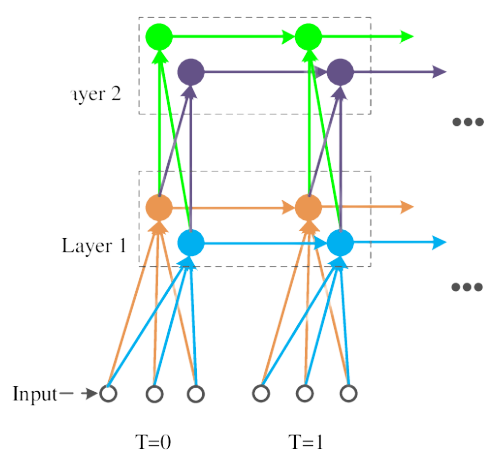
\includegraphics[scale=0.45]{gambar/indrnn.png}
  % Keterangan gambar yang diinputkan
  \caption{Ilustrasi IndRNN \parencite{8}}
  % Label referensi dari gambar yang diinputkan
  \label{fig:indrnn}
\end{figure}

IndRNN merupakan salah satu variasi \emph{deep learning} hasil pengembangan RNN yang bisa mengetahui pola temporal. IndRNN ini
diperlihatkan oleh Shuali Li et al. (2019). IndRNN memperkenalkan gagasan independensi di antara unit-unit waktu dalam jaringan rekuren,
sehingga setiap unit rekuren dapat beroperasi secara mandiri tanpa ketergantungan langsung pada unit-unit sebelumnya atau sesudahnya.
sedangkan pada RNN, setiap neuron terkait satu dengan lainnya dalam satu layer sesuai gambar \ref{fig:indrnn}. Pemrosesan neuron yang
independen ini memungkinkan IndRNN untuk memproses urutan panjang dengan menggunakan parameter yang sama pada setiap unit rekuren.
Keunggulan IndRNN terletak pada kemampuannya untuk memproses urutan waktu yang panjang dengan menggunakan parameter yang lebih efisien
dan menghindari \emph{vanishing gradient problem} yang sering terjadi pada RNN tradisional.



\section{\emph{Long Short Terms Memory} (LSTM)}

\begin{figure} [ht] \centering
  % Nama dari file gambar yang diinputkan
  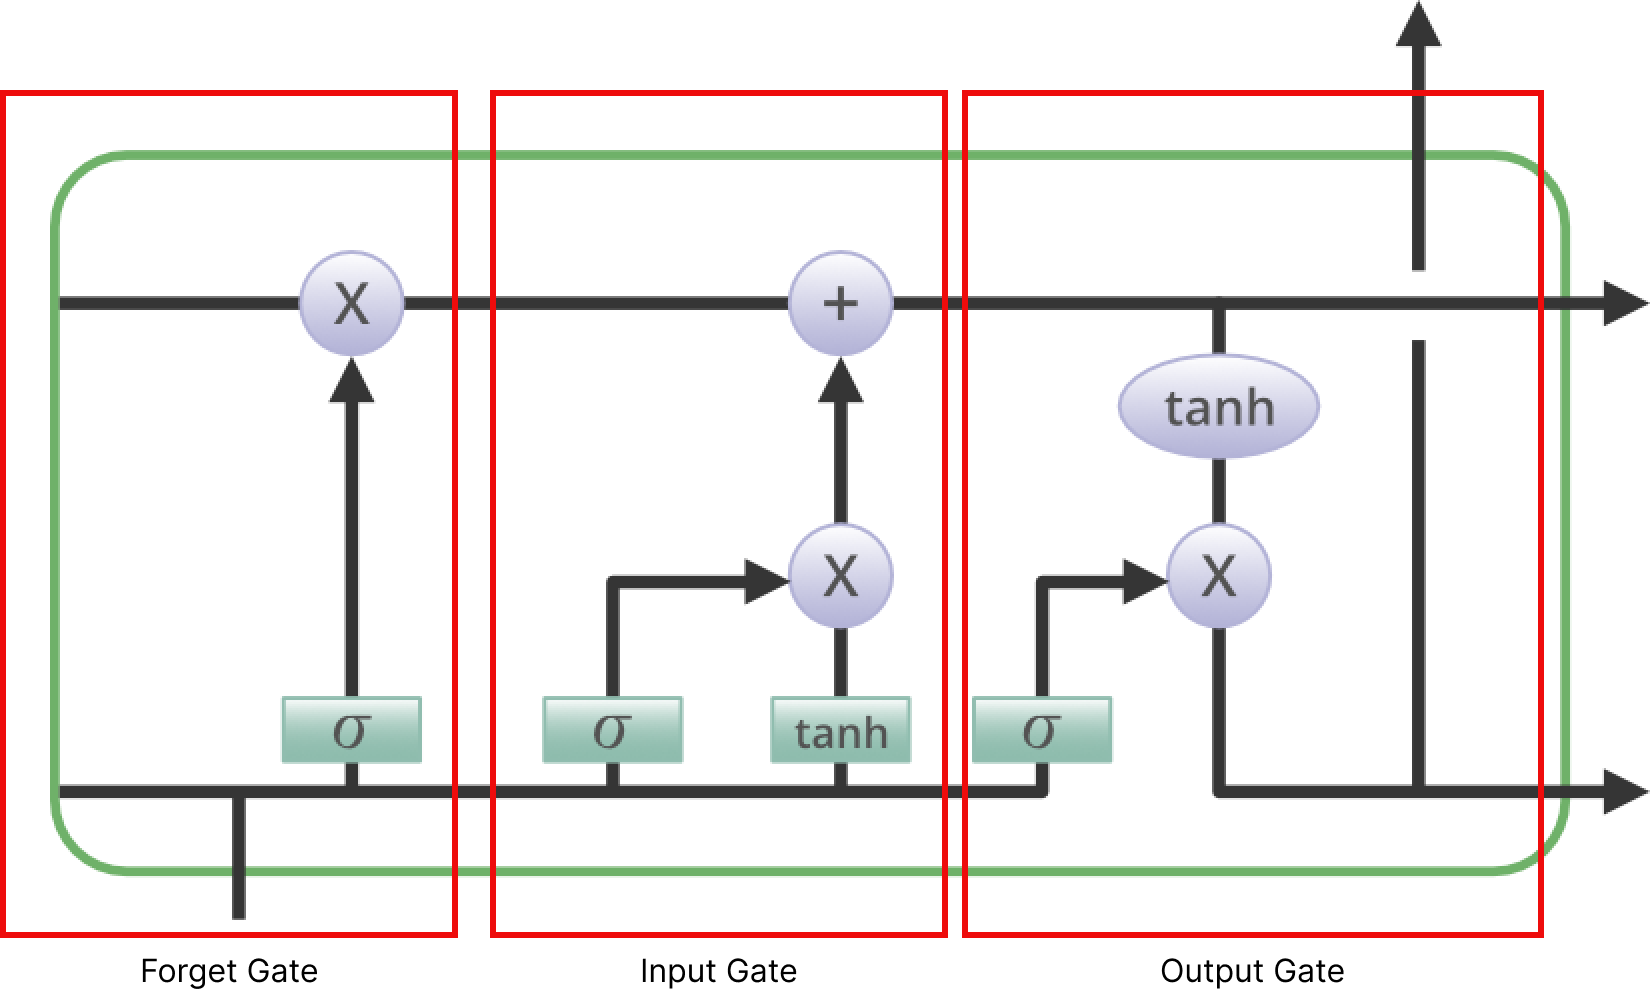
\includegraphics[scale=0.2]{gambar/LSTM.png}
  % Keterangan gambar yang diinputkan
  \caption{Struktur LSTM}
  % Label referensi dari gambar yang diinputkan
  \label{fig:LSTM}
\end{figure}

LSTM merupakan pengembangan atau salah satu jenis dari algoritma RNN
(\emph{Recurrent Neural Network}) yaitu dengan menambahkan memory cell yang dapat menyimpan
informasi untuk jangka waktu yang lama \parencite{26}. LSTM diajukan sebagai solusi
untuk mengatasi masalah \emph{vanishing gradient} yang terjadi saat memproses data berurutan
yang panjang saat menggunakan RNN. LSTM memiliki kemampuan untuk mengingat informasi
yang telah disimpan dalam jangka waktu panjang dan menghapus informasi yang tidak
relevan sehingga memungkinkannya untuk lebih efisien memproses, memprediksi, dan mengklasifikasikan
data berdasarkan urutan waktu tertentu. LSTM juga melibatkan proses backpropagation untuk melatih dan
memperbarui bobot-bobotnya. Gradien dihitung mundur melalui waktu untuk memperbarui bobot-bobot secara efisien.

Sistem LSTM terdiri dari empat gerbang, yaitu masukan (\emph{input gate}), gerbang
lupa (\emph{forget gate}), gerbang dan gerbang keluaran (\emph{output gate}) \parencite{27}.
Setiap gerbang memiliki peran dan tugasnya sendiri dalam mengumpulkan,
mengklasifikasi, dan memproses data. Selain memiliki empat gerbang tersebut,
LSTM juga dilengkapi dengan sel memori internal. Berikut penjelasan rinci mengenai komponen-komponen
pada LSTM:

\begin{enumerate}[nolistsep]
  \item Gerbang Input (\emph{Input Gate})

        Gerbang input mengontrol seberapa banyak informasi baru harus
        dimasukkan ke dalam sel memori. Ini melibatkan penggunaan fungsi
        aktivasi sigmoid untuk menghasilkan vektor bobot yang memperkirakan
        tingkat pentingnya informasi baru.

  \item Gerbang Lupa (\emph{Forget Gate})

        Gerbang lupa menentukan seberapa banyak informasi lama dalam sel
        memori harus dilupakan. Ini juga menggunakan fungsi aktivasi sigmoid
        untuk menghasilkan vektor bobot yang menentukan sejauh mana informasi
        lama harus dihapus atau dipertahankan.

  \item Sel Memori

        Sel memori merupakan komponen sentral dalam LSTM. Ini berfungsi
        sebagai "memori" jangka panjang yang dapat menyimpan dan mengingat
        informasi dalam urutan data. Sel memori dikontrol oleh gerbang input
        dan gerbang lupa untuk memperbarui dan mempertahankan informasi yang
        relevan.

  \item Gerbang Keluaran (\emph{Output Gate})

        Gerbang keluaran mengatur sejauh mana informasi dalam sel memori harus
        diungkapkan ke luar. Fungsi aktivasi sigmoid digunakan untuk menghasilkan
        vektor bobot yang mengontrol jumlah informasi yang dilewatkan.
\end{enumerate}

\section{\emph{Support Vector Machine} (SVM)}

SVM (\emph{Support Vector Machine}) adalah sebuah algoritma pembelajaran mesin yang
digunakan untuk tugas klasifikasi dan regresi. SVM menciptakan sebuah
hiperplane atau sebuah garis pemisah yang optimal dalam ruang fitur untuk
memisahkan data menjadi kelas yang berbeda. \parencite{28}

\begin{figure} [ht] \centering
  % Nama dari file gambar yang diinputkan
  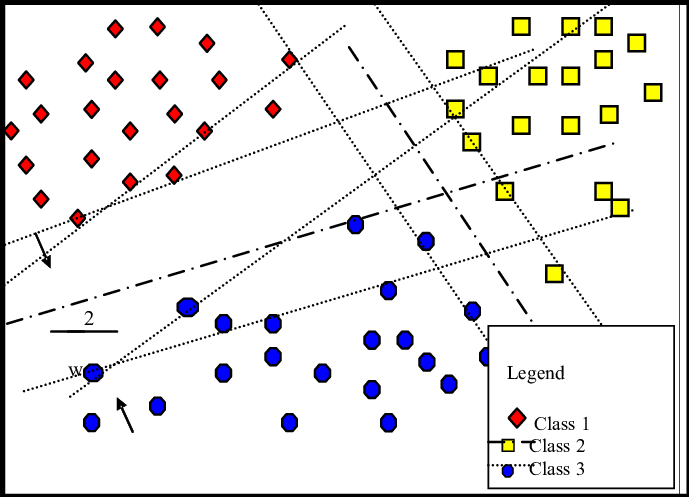
\includegraphics[scale=0.35]{gambar/SVM.png}
  % Keterangan gambar yang diinputkan
  \caption{SVM multiklas}
  % Label referensi dari gambar yang diinputkan
  \label{fig:SVM}
\end{figure}

\begin{enumerate}[nolistsep]
  \item Klasifikasi Linear:

        SVM memiliki kemampuan untuk melakukan klasifikasi linear, di mana
        algoritma ini mencari hiperplane yang secara optimal memisahkan dua kelas
        data. Hiperplane tersebut dapat berupa garis atau bidang yang berfungsi
        sebagai pemisah. SVM berupaya menemukan hiperplane dengan margin terbesar
        di antara dua kelas, yaitu jarak terpendek antara hiperplane dan titik-titik
        data terdekat dari masing-masing kelas.

  \item Kernel:

        SVM juga memiliki kemampuan untuk memodelkan hubungan non-linear antara
        fitur-fitur dengan menggunakan kernel. Kernel merupakan suatu fungsi
        yang mengubah data ke dalam ruang fitur yang memiliki dimensi lebih
        tinggi. Dalam ruang fitur yang lebih tinggi tersebut, SVM mencari
        hiperplane linier yang mampu memisahkan data secara optimal. Beberapa
        jenis kernel yang sering digunakan meliputi kernel linier, kernel
        polinomial, dan kernel radial basis function (RBF).

  \item Support Vectors:

        Support vectors adalah titik-titik data yang terletak pada atau dekat
        hiperplane pembatas. SVM menggunakan support vectors ini untuk
        menentukan hiperplane yang optimal. Hanya support vectors yang
        mempengaruhi posisi dan bentuk hiperplane, sementara titik-titik data
        lainnya tidak berperan dalam pembentukan hiperplane.

  \item Regularisasi dan Penalti:

        SVM menerapkan konsep regularisasi untuk mencegah overfitting.
        Parameter C dalam SVM mengatur keseimbangan antara mencapai margin
        maksimum dan mengurangi jumlah pelanggaran batas pemisah
        (misclassification). Semakin besar nilai C, semakin besar penalti
        yang diberikan untuk pelanggaran batas pemisah. Dengan demikian,
        nilai C yang lebih tinggi cenderung menghasilkan model yang lebih
        ketat dengan margin yang lebih sempit, sementara nilai C yang lebih
        rendah dapat memungkinkan adanya pelanggaran batas pemisah yang lebih
        besar.

  \item Regresi:

        Selain untuk klasifikasi, SVM juga dapat diterapkan dalam tugas
        regresi. Dalam SVM regresi, tujuannya adalah untuk membangun sebuah
        model yang dapat mendekati fungsi target dengan cara meminimalkan
        kesalahan antara output model dan target sebanyak mungkin. SVM regresi
        berusaha untuk menciptakan sebuah hiperplane yang memiliki margin
        terbesar di sekitar titik-titik data yang ada.
\end{enumerate}

\cleardoublepage

% Bab 3 metodologi
\chapter{METODOLOGI}
\label{chap:desainimplementasi}

% Ubah bagian-bagian berikut dengan isi dari desain dan implementasi

Pada bab metodologi akan dijelaskan mengenai bagaimana cara sistem ini
dibuat. Tujuan dari sistem ini adalah membuat model klasifikasi
tingkat kantuk seseorang dengan parameter EAR dan MAR menggunakan IndRNN
dengan \emph{output} 3 kelas berbeda.

\section{Metode yang digunakan}

% Contoh input gambar dengan format *.jpg
\begin{figure} [H] \centering
      % Nama dari file gambar yang diinputkan
      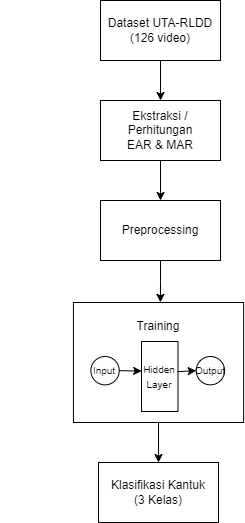
\includegraphics[scale=0.75]{gambar/metodologi.png}
      % Keterangan gambar yang diinputkan
      \caption{Diagram alur model}
      % Label referensi dari gambar yang diinputkan
      \label{fig:metodologi}
\end{figure}

% Contoh penggunaan referensi dari gambar yang diinputkan
Pada diagram yang tertera di Gambar \ref{fig:metodologi}. Didapatkan proses sebagai berikut:
\subsection{Pengumpulan Data}
Dataset UTA-RLDD digunakan sebagai sumber data input. Setiap video dalam kumpulan data ini memiliki perkiraan durasi
10 menit. Pengumpulan data dilakukan secara diseleksi secara manual. Dataset UTA-RLDD memiliki subjek video yang sangat beragam mulai
dari jenis kelamin, etnis, kegiatan yang dilakukan, ukuran video, keberadaan rambut wajah, dan pemakaian kacamata.
Terdapat beberapa video yang tidak bisa terbuka sehingga perlu dilakukan penyaringan data. Adapun kriteria dari
data yang dipilih adalah:
\begin{enumerate}[nolistsep]
      \item Video memiliki fps mendekati 30fps.
      \item Video memiliki jumlah frame diatas 16200.
      \item Video memiliki pencahayaan yang baik.
\end{enumerate}

\subsection{Ekstraksi Fitur}

\begin{figure} [H] \centering
      % Nama dari file gambar yang diinputkan
      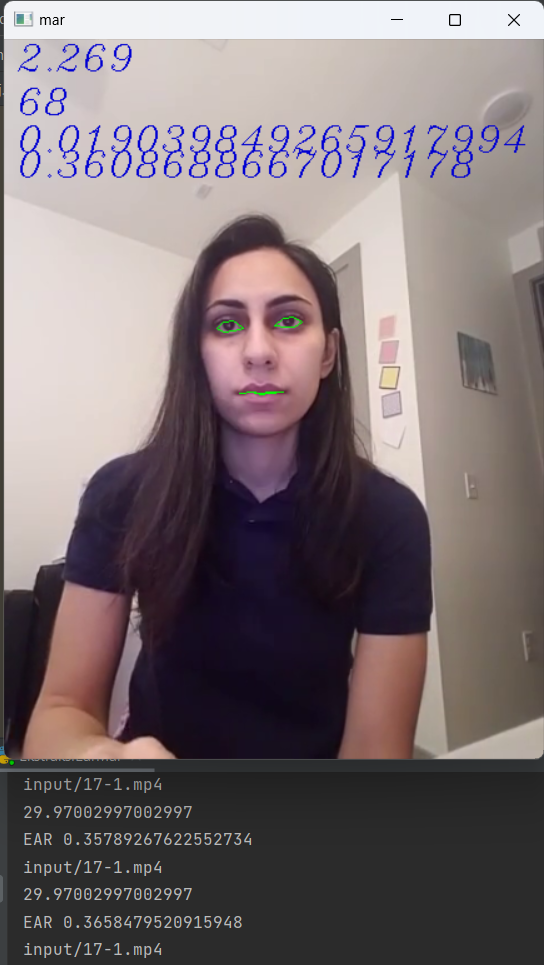
\includegraphics[scale=0.65]{gambar/ekstraksi.png}
      % Keterangan gambar yang diinputkan
      \caption{Proses ekstraksi nilai EAR dan MAR}
      % Label referensi dari gambar yang diinputkan
      \label{fig:ekstraksi}
\end{figure}

Ekstraksi fitur pada tiap video yang telah terpilih dilakukan secara lokal dengan bantuan IDE PyCharm edisi 2021.3.3.
Library Dlib menggunakan pendekatan berbasis fitur untuk mendeteksi landmark wajah. Algoritma pada library Dlib menggunakan
metode Histogram of Oriented Gradients (HOG) yang dikombinasikan dengan \emph{Support Vector Machines} (SVM) untuk mengenali pola wajah.
Deteksi wajah ini akan menghasilkan kotak pembatas (\emph{bounding box}) yang mengelilingi wajah dalam video. Setelah mendeteksi wajah,
langkah selanjutnya adalah menggunakan prediktor landmark Dlib untuk mengidentifikasi titik-titik landmark pada wajah.

Prediktor landmark menggunakan metode regresi untuk memprediksi koordinat titik landmark pada wajah berdasarkan fitur-fitur yang terlihat
dalam gambar. Prediktor ini mengambil gambar wajah yang terdeteksi sebagai input dan menghasilkan koordinat landmark yang sesuai.
Koordinat 68 titik landmark ini mencakup fitur-fitur seperti mata, hidung, mulut, dan sebagainya \parencite{13}. Setiap titik landmark
direpresentasikan oleh sepasang koordinat (x, y) yang menunjukkan posisinya dalam gambar seperti gambar \ref{fig:ekstraksi}.

Fitur-fitur yang diekstraksi pada tiap video yaitu nilai dari EAR dan MAR. Rumus \ref{eq:EAR} digunakan untuk mendapatkan
nilai EAR serta rumus \ref{eq:MAR} untuk mendapatkan nilai MAR. Rumus-rumus tersebut kemudian dimasukkan ke dalam program
sehingga menghasilkan data berupa csv yang berisi nilai EAR dan MAR dari tiap frame dalam setiap video. Nilai dari EAR dan MAR,
akan didapatkan pada tiap frame berdasarkan waktu.

\subsection{\emph{Preprocessing Data}}
Preprocessing data dilakukan menggunakan GoogleColab. Preprocessing data dilakukan untuk untuk meningkatkan kualitas data, mengurangi noise, dan membuat data siap digunakan untuk
pelatihan model. Tahapan preprocessing data yang telah dilakukan dalam penelitian ini adalah mengatasi data kosong, penyetaraan jumlah
data dan pemberian label, melakukan standarisasi data, serta melakukan kostumisasi pada data sehingga cocok digunakan untuk IndRNN.
Tahapan-tahapat tersebut dapat digambarkan menjadi gambar \ref{fig:preprocessing}:

% \newpage
\begin{figure} [H] \centering
      % Nama dari file gambar yang diinputkan
      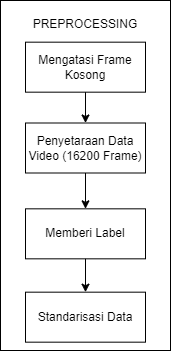
\includegraphics[scale=0.8]{gambar/preprocessing.png}
      % Keterangan gambar yang diinputkan
      \caption{Diagram Preprocessing Data}
      % Label referensi dari gambar yang diinputkan
      \label{fig:preprocessing}
\end{figure}

\begin{enumerate}[nolistsep]
      \item Interpolasi Linear

            Terdapat beberapa frame dari video yang landmark wajahnya
            tidak terdeteksi sehingga menyebabkan koordinat landmark wajah bernilai NaN.
            Interpolasi linear diperlukan untuk memperkirakan nilai di antara dua titik data yang diketahui.
            Interpolasi linear mengacu pada estimasi nilai di antara dua titik data yang diberikan
            berdasarkan garis lurus yang menghubungkan kedua titik tersebut. Konsep dasar interpolasi
            linear adalah menggunakan persamaan garis untuk memperkirakan nilai di antara dua titik data.
            Persamaan garis linear dinyatakan sebagai persamaan \ref{eq:interpolasi}:

            \begin{equation}
                  % Label referensi dari persamaan yang dibuat
                  \label{eq:interpolasi}
                  % Baris kode persamaan yang dibuat
                  y = mx + c
            \end{equation}

            Setelah nilai koordinat tiap frame tidak ada yang bernilai NaN maka nilai EAR dan MAR dapat kembali dihitung
            menggunakan hasil interpolasi koordinat titik-titik yang ada pada mata dan mulut dengan memasukkannya
            pada rumus \ref{eq:EAR} dan rumus \ref{eq:MAR}.

      \item Penyetaraan Jumlah Data dan Labeling

            Jumlah frame yang ada pada tiap video tidaklah sama oleh karena itu diperlukan pemotongan jumlah frame pada tiap video
            sehingga jumlah framenya dapat seragam yaitu 16200 frame tiap video. Ketika jumlah frame tiap video sudah seragam maka
            diberikanlah label yang sama pada tiap frame dalam satu video. Data-data tersebut kemudian dijadikan dalam satu csv
            sehingga lebih mudah untuk melakukan tahap preprocessing data selanjutnya.

      \item Normalisasi Standard Scaler

            Metode normalisasi standard scaler umum digunakan dalam preprocessing data. Tujuannya adalah untuk
            mentransformasikan data sehingga memiliki mean (rerata) nol dan deviasi standar satu. Normalisasi standard
            scaler dapat membantu meningkatkan performa model serta menghilangkan perbedaan skala antar fitur dalam dataset.
            Dengan demikian, semua fitur akan memiliki skala yang serupa, yang memudahkan perbandingan dan interpretasi data.
            Normalisasi data dengan fungsi Standard Scaler dapat diakses melalui library sklearn. Cara kerja dari normalisasi
            ini adalah mengganti nilai tersebut dengan nilai yang dihasilkan melalui rumus \ref{eq:StandardScaler}.

      \item Sliding Window

            \begin{figure} [H] \centering
                  % Nama dari file gambar yang diinputkan
                  
\includegraphics[scale=0.15]{gambar/PotongData.png}
                  % Keterangan gambar yang diinputkan
                  \caption{Ilustrasi pemotongan data}
                  % Label referensi dari gambar yang diinputkan
                  \label{fig:potong}
            \end{figure}
            Sebelum data dimasukkan ke sliding window, data terlebih dahulu dipisahkan menjadi data training dan data validasi atau
            testing. Dilakukan augmentasi pada data training dengan melakukan pemotongan data pada titik acu yang berbeda seperti gambar \ref{fig:potong}.
            Pemotongan dilakukan dari awal data, pemotongan yang dilakukan dari tengah data, dan pemotongan yang dilakukan
            dari akhir data. Sliding window digunakan sebagai teknik pemrosesan data untuk mempersiapkan data masukan yang lebih
            sesuai dengan kebutuhan model.  Metode sliding window digunakan karena inputan feature bersifat kontinu dan dalam satu
            feature terdapat banyak nilai yang tersimpan di dalam array.
\end{enumerate}

\subsection{\emph{Training Data}}
Pada proses klasifikasi yang menggunakan IndRNN nilai EAR dan MAR digunakan se-
bagai feature untuk proses training. Untuk output-nya sendiri akan terdiri dari 3 kelas yang
mengacu pada skala kantuk karolinska. 3 kelas tersebut terdiri dari: Kelas pertama (Waspada)
yaitu terdiri dari label kelas KSS 1 sampai 5 ( Amat Sangat Terjaga, Sangat Terjaga, Terjaga,
Sedikit terjaga, Tidak Terjaga namun Tidak ada Tanda Mengantuk), Kelas kedua (Kewaspadaan
Rendah) yaitu terdiri dari label kelas KSS 6 dan 7 ( Sedikit Mengantuk dan Mengantuk, perlu
sedikit usaha untuk terjaga), Kelas ketiga (Mengantuk) yaitu terdiri dari label kelas KSS 8 dan
9 (Mengantuk, perlu usaha untuk terjaga dan Sangat mengantuk, perlu usaha lebih untuk tetap
terjaga). Model klasifikasi dibuat menggunakan IndRNN sebagai klasifikatornya.

Model klasifikasi yang dibuat dengan arsitektur SVM, menggunakan parameter kernel RBF.
Kernel RBF (Radial Basis Function) atau juga dikenal sebagai Gaussian kernel adalah 
salah satu jenis kernel yang memetakan data ke dalam ruang fitur yang memiliki dimensi tak 
terhingga. Kernel RBF memberikan bobot pada setiap titik data berdasarkan jaraknya dari pusat. 
Semakin dekat titik data dengan pusat, semakin besar bobotnya. Dalam kernel RBF, bobot jarak 
dihitung dengan menggunakan fungsi Gaussian, yang menurun secara eksponensial dengan 
jarak. Kernel RBF digunakan untuk memodelkan hubungan non-linear antara fitur-fitur dalam 
data. Dengan melakukan pemetaan data ke dalam ruang fitur yang memiliki dimensi tak 
terhingga, kernel RBF memungkinkan SVM untuk menemukan hiperplane non-linear yang 
dapat memisahkan kelas-kelas data dengan lebih baik.

Berikut adalah gambaran arsitektur IndRNN yang digunakan:

\begin{figure} [H] \centering
      % Nama dari file gambar yang diinputkan
      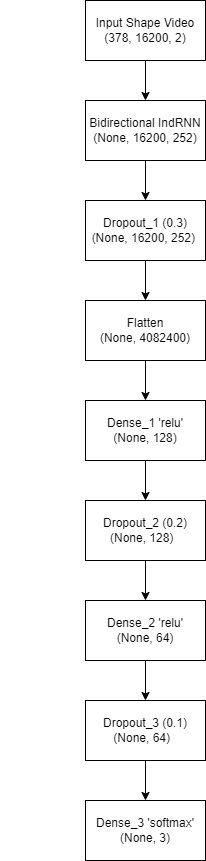
\includegraphics[scale=0.7]{gambar/arsitekturmodel.png}
      % Keterangan gambar yang diinputkan
      \caption{Arsitektur Model Klasifikasi IndRNN}
      % Label referensi dari gambar yang diinputkan
      \label{fig:arsitekturmodel}
\end{figure}

\begin{enumerate}[nolistsep]
      \item Input: IndRNN menerima input berupa urutan data, seperti urutan waktu dalam bentuk deret waktu atau urutan spasial dalam citra.
            Setiap elemen dalam urutan dianggap sebagai input pada satu waktu tertentu. IndRNN memiliki input yang berpentuk 3 dimensi jika
            pada penelitian yang dilakukan, bentuk input modelnya adalah (353, 16200, 2).

      \item Hidden Units: Setiap unit rekuren dalam IndRNN memiliki \emph{hidden state} atau \emph{output} yang dihasilkan dari pemrosesan input dan
            bobotnya. Hidden state ini merepresentasikan informasi yang dihasilkan oleh unit rekuren pada waktu tertentu. Model klasifikasi
            pada penelitian ini memiliki 126 hidden units.

      \item Weight Matrix: Setiap unit rekuren dalam IndRNN menggunakan \emph{weight matrix} (matriks bobot) yang berkorelasi dengan dirinya sendiri.
            Matriks bobot ini digunakan dalam operasi perkalian untuk menghitung \emph{output} unit rekuren pada waktu tertentu.

      \item Non-linear Activation: Setelah melakukan operasi perkalian dengan input dan bobotnya, output dari setiap unit rekuren umumnya
            melewati fungsi aktivasi non-linear, seperti fungsi ReLU, untuk memperkenalkan sifat non-linearitas dalam jaringan.

      \item \emph{Output}: IndRNN dapat menghasilkan output pada setiap waktu tertentu berdasarkan hidden state dari unit-unit rekuren. \emph{Output} ini
            dapat digunakan untuk klasifikasi kantuk yang menghasilkan 3 jenis kelas berbeda.

\end{enumerate}

Berikut merupakan gambaran arsitektur LSTM yang digunakan sebagai model
klasifikasi kantuk:
\begin{figure} [H] \centering
      % Nama dari file gambar yang diinputkan
      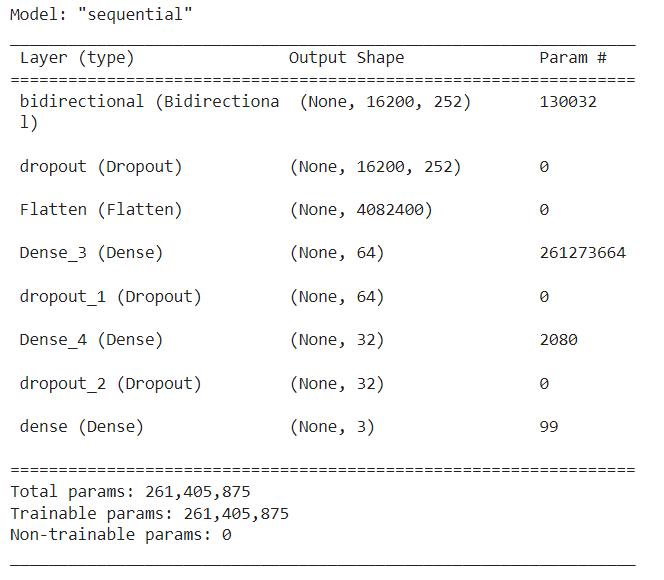
\includegraphics[scale=0.7]{gambar/arsitekturLSTM.png}
      % Keterangan gambar yang diinputkan
      \caption{Arsitektur Model Klasifikasi LSTM}
      % Label referensi dari gambar yang diinputkan
      \label{fig:arsitekturLSTM}
\end{figure}

\newpage
Berikut merupakan tabel hyperparameter yang digunakan untuk membangun model klasifikasi pada penelitian ini:

\begin{longtable}{|c|c|}
      \caption{Pengaturan Hyperparameter Model Klasifikasi}
      \label{tb:Hyperparameter}                             \\
      \hline
      \rowcolor[HTML]{C0C0C0}
      \textbf{Hyperparameter}              & \textbf{Nilai} \\
      \hline
      Arsitektur Model (IndRNN, LSTM, SVM) & 126 unit       \\
      Regularisasi L2                      & 1e-07          \\
      Dropout\_1                           & 0.3            \\
      Dropout\_2                           & 0.2            \\
      Dropout\_3                           & 0.1            \\
      activation                           & ReLu           \\
      output activation                    & softmax        \\
      solver                               & adam           \\
      initial learning rate                & 0.000025       \\
      \hline
\end{longtable}

\begin{enumerate}[nolistsep]
      \item Regularisasi L2

            Regularisasi L2 adalah salah satu metode regularisasi dalam pembelajaran mesin. Tujuan dari digunakannya regularisasi L2
            adalah untuk mengendalikan kompleksitas model dan mencegah overfitting. Regulasi L2 biasa digunakan pada data yang kompleks yang
            menyebabkan kondisi model terlalu "menghafal" data pelatihan dan tidak mampu menggeneralisasi dengan baik pada data yang
            belum pernah dilihat sebelumnya. Regularisasi L2 membantu mencegah overfitting dengan mengurangi bobot yang besar, sehingga
            membatasi kapasitas model untuk "menghafal" data pelatihan dan memaksa model untuk fokus pada pola yang lebih umum dan general.
            Regulasi L2 juga dapat membuat model lebih stabil dan konsisten dengan mengendalikan varians serta mengendalikan kemampuan model
            dengan dengan memberikan penalti pada bobot yang lebih besar, sehingga mendorong model untuk menggunakan representasi yang lebih
            sederhana dan parsial dari data.

      \item Fungsi Aktivasi Non-Linear

            Pada model klasifikasi kantuk dengan IndRNN, ReLU digunakan untuk memperkenalkan sifat non-linearitas dalam jaringan.
            Alasan digunakannya ReLU pada model klasifikasi karena implementasinya sederhana, perhitungan ReLU dapat dijalankan
            secara efisien di perangkat keras seperti GPU. ReLU dapat mengurangi masalah gradien yang cenderung menghilang
            (\emph{vanishing gradient}) saat mengalami backpropagation, terutama pada lapisan-lapisan terdalam. ReLU memungkinkan pelatihan
            model yang lebih cepat dan efisien. Fungsi aktivasi softmax digunakan pada lapisan dense terakhir dengan tujuan
            menghasilkan distribusi probabilitas yang menunjukkan kemungkinan setiap kelas sebagai output dari model.

      \item Optimisasi

            Optimisasi Adam (Adaptive Moment Estimation) adalah algoritma optimasi yang menggabungkan konsep dari optimizer RMSProp dan Momentum
            untuk menghasilkan tingkat konvergensi yang cepat dan efisien. Optimisasi Adam menghitung momen pertama dan kedua dari gradien. Momen
            pertama digunakan untuk mengestimasi kecepatan perubahan bobot, sedangkan momen kedua digunakan untuk mengestimasi kecepatan perubahan
            kecepatan perubahan bobot. Hal ini membantu algoritma untuk menyesuaikan langkah optimisasi berdasarkan gradien yang terkini dan
            mempertimbangkan sejarah gradien sebelumnya. Dengan melakukan penyesuaian learning rate berdasarkan estimasi momen, optimisasi Adam
            mampu menyesuaikan langkah optimisasi dengan lebih baik dan mengurangi dampak dari learning rate yang tidak tepat. Optimisasi Adam
            melibatkan regularisasi untuk mencegah overfitting pada model. Regularisasi dilakukan melalui metode L2 regularization.
            Optimizer Adam digunakan untuk mempercepat dan meningkatkan proses pelatihan model IndRNN, sehingga memungkinkan model
            untuk belajar pola yang lebih kompleks dan akurat dari data sequence yang ada.
\end{enumerate}

\subsection{Evaluasi Model}
Evaluasi model dilakukan untuk untuk memahami dan mengukur performa model dalam melakukan prediksi pada dataset.
Beberapa metrik evaluasi yang umum digunakan adalah Confusion Matrix, Akurasi,
Presisi, Recall, dan F1-Score. Semakin tinggi nilai precision, recall, dan f1 score maka semakin baik performa model. Nilai loss yang
mendekati 0 menandakan hasil probabilitas prediksi mendekati nilai yang benar dan juga sebaliknya. Nilai
yang benar pada confusion matrix dapat diliat dari garis diagonalnya. Tahapan skenario evaluasi model
meliputi beberapa poin berikut:

\begin{enumerate}[nolistsep]
      \item Pengujian Performa Model IndRNN dengan Confusion Matrix
      \item Pengujian Performa Model IndRNN dengan Akurasi, Presisi, Recall, dan F1-Score
      \item Pengujian Performa Model LSTM dengan Confusion Matrix
      \item Pengujian Performa Model LSTM dengan Akurasi, Presisi, Recall, dan F1-Score
      \item Pengujian Performa Model SVM dengan Confusion Matrix
      \item Pengujian Performa Model SVM dengan Akurasi, Presisi, Recall, dan F1-Score
\end{enumerate}

\subsection{Testing Model}
Testing model digunakan untuk mengetahui kinerja model yang telah dibuat. Testing model
dilakukan dengan menggunakan video yang ada pada dataset DROZY. Video yang ada pada dataset
diproses dahulu seperti video yang berasal dari dataset UTA-RLDD sehingga menghasilkan
data yang sesuai. Video yang memiliki jumlah frame yang kurang dari 16200 tidak digunakan
untuk melakukan testing model.

\section{Data dan peralatan yang digunakan}
\subsection{Dataset UTA-RLDD}

\begin{figure} [H] \centering
      % Nama dari file gambar yang diinputkan
      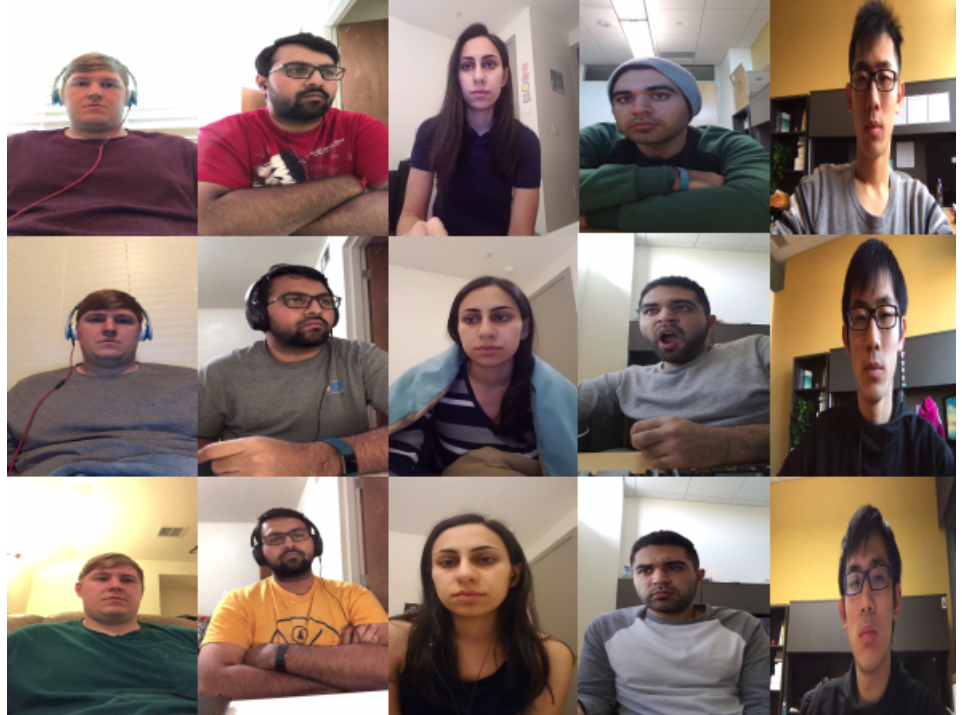
\includegraphics[scale=0.4]{gambar/utarldd.png}
      % Keterangan gambar yang diinputkan
      \caption{Sampel data UTA-RLDD dalam status waspada (baris pertama), waspada rendah (baris kedua), dan mengantuk (baris ketiga) \parencite{14}}
      % Label referensi dari gambar yang diinputkan
      \label{fig:utarldd}
\end{figure}

UTA-RLDD (\emph{The University of Texas at Arlington Real-Life Drowsiness Dataset}) dibuat untuk tugas deteksi kantuk \emph{multi-stages}.
Dataset ini terditi dari 60 subjek sehat (51 laki-laki dan 9 perempuan) dengan usia diatas 18 tahun. Panjang durasi jumlah
video yang ada sekitar 30jam RGB dengan fps hingga 30. Subjek diminta untuk mengambil 3 buah video mereka delam 3 kondisi
kantuk yang berbeda dengan durasi masing-masing sekitar 10 menit\parencite{14}. Ketiga kelas tersebut dijelaskan kepada para peserta sebagai
berikut:

1) Waspada: Salah satu dari tiga kondisi pertama yang disorot dalam tabel KSS dengan nilai 1 hingga 3 dimana subyek dalam
keadaan masih waspada dan benar-benar sadar sehingga mereka dapat mengemudi selama berjam-jam dengan mudah.

2) Kewaspadaan Rendah : Memiliki nilai 6 dan 7 dalam tabel KSS dimana ketika beberapa tanda kantuk muncul, atau kantuk
hadir tetapi tidak diperlukan upaya untuk tetap waspada. Subjek mungkin dapat mengemudi dalam kondisi ini tapi tidak dianjurkan.

3) Mengantuk : Keadaan ini berarti subjek harus secara aktif berusaha untuk tidak tertidur dengan nilai 8 dan 9 pada Tabel KSS.

\subsection{Dataset DROZY}

\begin{figure} [H] \centering
      % Nama dari file gambar yang diinputkan
      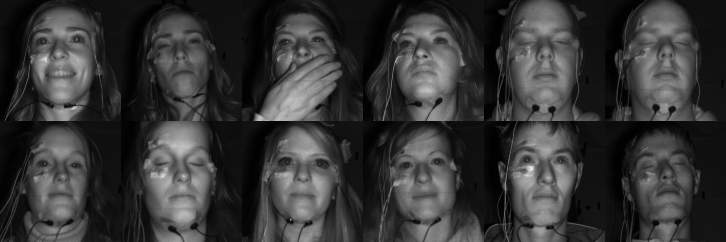
\includegraphics[scale=0.4]{gambar/DROZY.png}
      % Keterangan gambar yang diinputkan
      \caption{Sampel data DROZY \parencite{29}}
      % Label referensi dari gambar yang diinputkan
      \label{fig:DROZY}
\end{figure}

Database DROZY berisi berbagai tipe data yang berhubungan dengan kantuk (sinyal, gambar, dan sebagainya). Database ini
bertujuan untuk membantu para peneliti untuk melakukan eksperimen, mengembangkan, serta mengevaluasi sistem pada monitoring
kantuk. Data yang ada di DROZY diambil dari 14 partisipan (3 pria, 11 wanita) yang melakukan simulasi berkendara selama
10 menit dalam kondisi kurang tidur yang disebabkan oleh bangun yang berkepanjangan. Untuk setiap subjek, dan untuk setiap
PVT, database berisi data tersinkronisasi waktu dengan sempurna berikut:

1)	Nilai KSS

2)	PVT data

3)	Polysomnography signals

4)	Kinect V2 sensor videos

5)	Face Landmarks (Manual)

6)	Face Landmarks (Otomatis)

7)	Index Interpolasi

\subsection{Peralatan}

Berikut merupakan peralatan yang diperlukan untuk membangun model klasifikasi kantuk dengan menggunakan IndRNN:

\begin{enumerate}[nolistsep]
      \item Laptop yang digunakan untuk mengumpulkan data, training, evaluasi, hingga testing memiliki spesifikasi Intel(R)
            Core(TM) i7-8565U CPU @1.80GHz 1.99 GHz, 16 GB LPDDR3 RAM, 512GB M.2 NVMe PCIe SSD, NVIDIA GeForce MX150 with
            2GB GDDR5 VRAM, Windows 10 Pro 64-bit.
      \item GoogleColab merupakan produk Google research berbasis Cloud yang dapat digunakan secara gratis. Untuk menjalankan
            training model sistem klasifikasi menggunakan IndRNN dibutuhkan TPU serta \emph{Runtime Shape High-RAM} karena jumlah
            data yang ditraining cukup besar.
      \item PyCharm edisi 2021.3.3 digunakan untuk melakukan ekstraksi data secara lokal. PyCharm merupakan IDE (\emph{Integrated Development Environment})
            yang biasa digunakan untuk membangun model \emph{machine learning} yang menawarkan kemudahan untuk membangun \emph{environment} berbeda sesuai
            kebutuhan.

\end{enumerate}


\cleardoublepage

% Bab 4 pengujian dan analisis
\chapter{HASIL DAN PEMBAHASAN}
\label{chap:pengujiananalisis}

% Ubah bagian-bagian berikut dengan isi dari pengujian dan analisis

Pada penelitian ini akan dipaparkan hasil dan pembahasan dari proses-proses yang telah dilakukan pada
bab metodologi. Hasil pembahasan yang ada pada bab ini diharapkan agar dapat ditarik suatu kesimpulan
dari pelaksanaan tugas akhir yang telah dilakukan.

\section{Hasil Pengumpulan Data}
\label{sec:skenariopengujian}

Video yang digunakan sebagai masukan dari model yang dibuat, diambil dari dataset UTA-RLDD. Banyak video yang perlu disaring
pada dataset ini guna menghasilkan data yang cukup baik. Video dengan fps yang mendekati 30 fps saja yang dapat digunakan sebagai
data masukan model. Didapatkan sebanyak 42 video pada setiap kelas seperti gambar \ref{tb:JumlahVideo} sehingga jumlah video
yang dapat diekstraksi datanya berjumlah 126 video. Video yang ada pada dataset ini terbagi menjadi 3 kelas berbeda yaitu
kelas 1 (Waspada), kelas 2 (Kewaspadaan Rendah), serta kelas 3 (Mengantuk). Subjek pada video yang diambil terdiri dari pria
dan wanita yang berasal dari berbagai etnis serta sejumlah subjek yang ada pada video memakai kacamata serta memiliki bulu
yang lebat di wajah. Berikut merupakan gambar sebaran jumlah video berdasarkan masing-masing kelas:

\begin{longtable}{|c|c|}
  \caption{Sebaran Video Tiap Kelas}
  \label{tb:JumlahVideo}                 \\
  \hline
  \rowcolor[HTML]{C0C0C0}
  \textbf{Kelas} & \textbf{Jumlah Video} \\
  \hline
  1              & 42                    \\
  2              & 42                    \\
  3              & 42                    \\
  \hline
\end{longtable}

\section{Hasil Ekstraksi Fitur}
Ekstraksi fitur dilakukan secara lokal dengan bantuan IDE PyCharm edisi 2021.3.3 menghasilkan
koordinat setiap titik pada mata maupun mulut berupa sumbu (x, y). Titik-titik koordinat tersebut nantinya
akan digunakan untuk melakukan perhitungan sesuai dengan rumus \ref{eq:EAR} untuk menghasilkan nilai EAR
serta rumus \ref{eq:MAR} untuk menghasikan nilai MAR. Berikut merupakan gambaran data-data yang didapat
setelah melakukan ekstraksi fitur:

\begin{longtable}{|c|c|c|c|}
  \caption{Deskripsi Data Hasil Ekstraksi Fitur}
  \label{tb:DeskripsiData}                                                                          \\
  \hline
  \rowcolor[HTML]{C0C0C0}
  \textbf{No} & \textbf{Nama Kolom} & \textbf{Tipe Data} & \textbf{Deskripsi}                       \\
  \hline
  1           & frame               & \textit{integer}   & Jumlah Frame                             \\
  2           & timestamp\_x        & \textit{float}     & Waktu (detik)                            \\
  3           & xl0\_x              & \textit{float}     & Titik x pada koordinat 36 Landmark Wajah \\
  4           & yl0\_x              & \textit{float}     & Titik y pada koordinat 36 Landmark Wajah \\
  5           & xl1\_x              & \textit{float}     & Titik x pada koordinat 37 Landmark Wajah \\
  6           & yl1\_x              & \textit{float}     & Titik y pada koordinat 37 Landmark Wajah \\
  7           & xl2\_x              & \textit{float}     & Titik x pada koordinat 38 Landmark Wajah \\
  8           & yl2\_x              & \textit{float}     & Titik y pada koordinat 38 Landmark Wajah \\
  9           & xl3\_x              & \textit{float}     & Titik x pada koordinat 39 Landmark Wajah \\
  10          & yl3\_x              & \textit{float}     & Titik y pada koordinat 39 Landmark Wajah \\
  11          & xl4\_x              & \textit{float}     & Titik x pada koordinat 40 Landmark Wajah \\
  12          & yl4\_x              & \textit{float}     & Titik y pada koordinat 40 Landmark Wajah \\
  13          & xl5\_x              & \textit{float}     & Titik x pada koordinat 41 Landmark Wajah \\
  14          & yl5\_x              & \textit{float}     & Titik y pada koordinat 41 Landmark Wajah \\
  15          & xr0\_x              & \textit{float}     & Titik x pada koordinat 42 Landmark Wajah \\
  16          & yr0\_x              & \textit{float}     & Titik y pada koordinat 42 Landmark Wajah \\
  17          & xr1\_x              & \textit{float}     & Titik x pada koordinat 43 Landmark Wajah \\
  18          & yr1\_x              & \textit{float}     & Titik y pada koordinat 43 Landmark Wajah \\
  19          & xr2\_x              & \textit{float}     & Titik x pada koordinat 44 Landmark Wajah \\
  20          & yr2\_x              & \textit{float}     & Titik y pada koordinat 44 Landmark Wajah \\
  21          & xr3\_x              & \textit{float}     & Titik x pada koordinat 45 Landmark Wajah \\
  22          & yr3\_x              & \textit{float}     & Titik y pada koordinat 45 Landmark Wajah \\
  23          & xr4\_x              & \textit{float}     & Titik x pada koordinat 46 Landmark Wajah \\
  24          & yr4\_x              & \textit{float}     & Titik y pada koordinat 46 Landmark Wajah \\
  25          & xr5\_x              & \textit{float}     & Titik x pada koordinat 47 Landmark Wajah \\
  26          & yr5\_x              & \textit{float}     & Titik y pada koordinat 47 Landmark Wajah \\
  27          & ear\_x              & \textit{float}     & Nilai Kalkulasi EAR                      \\
  28          & x0\_x               & \textit{float}     & Titik x pada koordinat 60 Landmark Wajah \\
  29          & y0\_x               & \textit{float}     & Titik y pada koordinat 60 Landmark Wajah \\
  30          & x1\_x               & \textit{float}     & Titik x pada koordinat 61 Landmark Wajah \\
  31          & y1\_x               & \textit{float}     & Titik y pada koordinat 61 Landmark Wajah \\
  32          & x2\_x               & \textit{float}     & Titik x pada koordinat 62 Landmark Wajah \\
  33          & y2\_x               & \textit{float}     & Titik y pada koordinat 62 Landmark Wajah \\
  34          & x3\_x               & \textit{float}     & Titik x pada koordinat 63 Landmark Wajah \\
  35          & y3\_x               & \textit{float}     & Titik y pada koordinat 63 Landmark Wajah \\
  36          & x4\_x               & \textit{float}     & Titik x pada koordinat 64 Landmark Wajah \\
  37          & y4\_x               & \textit{float}     & Titik y pada koordinat 64 Landmark Wajah \\
  38          & x5\_x               & \textit{float}     & Titik x pada koordinat 65 Landmark Wajah \\
  39          & y5\_x               & \textit{float}     & Titik y pada koordinat 65 Landmark Wajah \\
  40          & x6\_x               & \textit{float}     & Titik x pada koordinat 66 Landmark Wajah \\
  41          & y6\_x               & \textit{float}     & Titik y pada koordinat 66 Landmark Wajah \\
  42          & x7\_x               & \textit{float}     & Titik x pada koordinat 67 Landmark Wajah \\
  43          & y7\_x               & \textit{float}     & Titik y pada koordinat 67 Landmark Wajah \\
  44          & mar\_x              & \textit{float}     & Nilai Kalkulasi MAR                      \\
  \hline
\end{longtable}

\section{Hasil Preprocessing}

Preprocessing data dilakukan untuk menyiapkan data pelatihan model sehingga dapat menghasilkan
model klasifikasi yang baik. Berikut hasil implementasikan praproses data pada pengembangan penelitian
diantaranya melakukan ekstraksi fitur, mengatasi data/frame kosong, melakukan penyetaraan jumlah data
dan labeling, melakukan normalisasi data, serta melakukan penyesuaian bentuk data.

\subsection{Hasil Interpolasi Data}
Video yang telah terpilih tidak selalu memiliki data yang lengkap pada tiap frame. Terdapat data yang
bernilai NaN dikarenakan koordinat landmark wajahnya tidak terdeteksi. Oleh karena itu digunakan interpolasi
linear untuk mengisi data yang nilainya NaN sehingga titik-titik koordinat yang dibutuhkan untuk menghitung
nilai EAR maupun MAR menjadi lengkap dan bisa mendapatkan nilai dari EAR maupun MAR itu sendiri. Berikut
merupakan contoh tabel data yang memiliki nilai NaN di dalamnya sebelum maupun setelah dilakukannya
interpolasi:

\begin{longtable}{|c|c|c|c|}
  \caption{Data Kosong Sebelum Interpolasi}
  \label{tb:NaNdata}                                                       \\
  \hline
  \rowcolor[HTML]{C0C0C0}
  \textbf{timestamp\_x} & \textbf{xl0\_x} & \textbf{...} & \textbf{mar\_x} \\
  \hline
  10.329                & 78              & ...          & 0.1197736075    \\
  10.362                & 78              & ...          & 0.1427218439    \\
  10.395                & NaN             & ...          & NaN             \\
  10.428                & NaN             & ...          & NaN             \\
  10.461                & 77              & ...          & 0.1290500622    \\
  10.494                & 77              & ...          & 0.1433720878    \\
  10.527                & 78              & ...          & 0.1215658232    \\
  \hline
\end{longtable}

\begin{longtable}{|c|c|c|c|}
  \caption{Data Kosong Setelah Interpolasi}
  \label{tb:noNaNdata}                                                     \\
  \hline
  \rowcolor[HTML]{C0C0C0}
  \textbf{timestamp\_x} & \textbf{xl0\_x} & \textbf{...} & \textbf{mar\_x} \\
  \hline
  10.329                & 78              & ...          & 0.1197736075    \\
  10.362                & 78              & ...          & 0.1427218439    \\
  10.395                & 78              & ...          & 0.05930266631   \\
  10.428                & 77              & ...          & 0.05930266631   \\
  10.461                & 77              & ...          & 0.1290500622    \\
  10.494                & 77              & ...          & 0.1433720878    \\
  10.527                & 78              & ...          & 0.1215658232    \\
  \hline
\end{longtable}


\subsection{Hasil Penyetaraan Data dan Labeling}
Panjang data yang didapatkan pada setiap video tidaklah sama seperti pada tabel \ref{tb:JumlahData}, oleh karena itu
perlu dilakukan penyetaraan panjang data pada tiap video sehingga dapat menjadi
inputan untuk model klasifikasi. Pada tahap ini hanya kolom ear\_x dan mar\_x
saja yang digunakan. Panjang data yang dibutuhkan adalah 16200 data tiap video.
Setelah jumlah data diseragamkan, maka data-data tersebut akan diberi label tiap
frame sesuai dengan label yang telah ditentukan oleh dataset UTA-RLDD. Berikut
merupakan tabel rincian jumlah data yang didapat yang ada pada setiap video:

\begin{longtable}{|c|c|c|c|c|c|c|c|c|}
  \caption{Jumlah Data Pada Tiap Video}
  \label{tb:JumlahData}                                                                                                                      \\
  \hline
  \rowcolor[HTML]{C0C0C0}
  \textbf{No} & \textbf{Video} & \textbf{Data} & \textbf{No} & \textbf{Video} & \textbf{Data} & \textbf{No} & \textbf{Video} & \textbf{Data} \\
  \hline
  1           & 13-1.csv       & 18234         & 43          & 10-2.csv       & 18620         & 85          & 10-3.csv       & 18866         \\
  2           & 35-1.csv       & 18027         & 44          & 13-2.csv       & 20477         & 86          & 13-3.csv       & 18486         \\
  3           & 59-1.csv       & 18089         & 45          & 59-2.csv       & 18169         & 87          & 34-3.csv       & 18388         \\
  4           & 7-1.csv        & 18016         & 46          & 19-2.csv       & 18035         & 88          & 35-3.csv       & 18340         \\
  5           & 21-1.csv       & 18151         & 47          & 21-2.csv       & 18031         & 89          & 59-3.csv       & 18095         \\
  6           & 19-1.csv       & 18029         & 48          & 9-2.csv        & 18367         & 90          & 7-3.csv        & 17939         \\
  7           & 9-1.csv        & 18172         & 49          & 34-2.csv       & 20693         & 91          & 20-3.csv       & 21437         \\
  8           & 60-1.csv       & 18054         & 50          & 60-2.csv       & 17533         & 92          & 19-3.csv       & 18064         \\
  9           & 42-1.csv       & 18021         & 51          & 35-2.csv       & 18022         & 93          & 21-3.csv       & 18055         \\
  10          & 5-1.csv        & 18410         & 52          & 56-2.csv       & 18354         & 94          & 9-3.csv        & 19816         \\
  11          & 8-1.csv        & 18158         & 53          & 42-2.csv       & 18122         & 95          & 60-3.csv       & 18581         \\
  12          & 10-1.csv       & 16417         & 54          & 40-2.csv       & 18036         & 96          & 5-3.csv        & 18050         \\
  13          & 56-1.csv       & 18355         & 55          & 36-2.csv       & 18792         & 97          & 8-3.csv        & 17989         \\
  14          & 14-1.csv       & 18386         & 56          & 5-2.csv        & 18062         & 98          & 56-3.csv       & 19417         \\
  15          & 15-1.csv       & 19301         & 57          & 7-2.csv        & 17886         & 99          & 14-3.csv       & 18692         \\
  16          & 22-1.csv       & 18221         & 58          & 14-2.csv       & 19742         & 100         & 15-3.csv       & 18483         \\
  17          & 1-1.csv        & 18055         & 59          & 15-2.csv       & 18541         & 101         & 22-3.csv       & 18316         \\
  18          & 2-1.csv        & 18263         & 60          & 22-2.csv       & 18266         & 102         & 1-3.csv        & 18012         \\
  19          & 17-1.csv       & 18121         & 61          & 1-2.csv        & 18033         & 103         & 2-3.csv        & 18124         \\
  20          & 12-1.csv       & 16919         & 62          & 2-2.csv        & 18106         & 104         & 3-3.csv        & 18480         \\
  21          & 23-1.csv       & 17567         & 63          & 8-2.csv        & 18048         & 105         & 17-3.csv       & 18212         \\
  22          & 20-1.csv       & 19122         & 64          & 3-2.csv        & 18514         & 106         & 23-3.csv       & 18187         \\
  23          & 25-1.csv       & 17992         & 65          & 17-2.csv       & 18245         & 107         & 25-3.csv       & 17987         \\
  24          & 26-1.csv       & 18489         & 66          & 12-2.csv       & 18838         & 108         & 26-3.csv       & 20849         \\
  25          & 27-1.csv       & 19724         & 67          & 20-2.csv       & 17957         & 109         & 27-3.csv       & 18627         \\
  26          & 30-1.csv       & 20439         & 68          & 23-2.csv       & 17286         & 110         & 30-3.csv       & 18251         \\
  27          & 36-1.csv       & 18694         & 69          & 25-2.csv       & 18016         & 111         & 36-3.csv       & 18728         \\
  28          & 37-1.csv       & 20483         & 70          & 26-2.csv       & 26445         & 112         & 37-3.csv       & 20396         \\
  29          & 38-1.csv       & 18056         & 71          & 27-2.csv       & 18774         & 113         & 39-3.csv       & 18158         \\
  30          & 39-1.csv       & 19376         & 72          & 30-2.csv       & 20846         & 114         & 40-3.csv       & 18029         \\
  31          & 40-1.csv       & 18060         & 73          & 37-2.csv       & 18551         & 115         & 41-3.csv       & 25166         \\
  32          & 41-1.csv       & 18839         & 74          & 38-2.csv       & 18097         & 116         & 42-3.csv       & 18030         \\
  33          & 43-1.csv       & 35818         & 75          & 39-2.csv       & 18173         & 117         & 43-3.csv       & 34975         \\
  34          & 48-1.csv       & 18913         & 76          & 43-2.csv       & 35936         & 118         & 46-3.csv       & 17773         \\
  35          & 47-1.csv       & 18027         & 77          & 48-2.csv       & 18183         & 119         & 47-3.csv       & 18340         \\
  36          & 58-1.csv       & 18054         & 78          & 47-2.csv       & 18022         & 120         & 54-3.csv       & 18944         \\
  37          & 54-1.csv       & 19107         & 79          & 58-2.csv       & 18302         & 121         & 58-3.csv       & 18244         \\
  38          & 49-1.csv       & 18191         & 80          & 49-2.csv       & 17917         & 122         & 50-3.csv       & 20013         \\
  39          & 50-1.csv       & 18174         & 81          & 50-2.csv       & 21683         & 123         & 51-3.csv       & 18494         \\
  40          & 51-1.csv       & 18182         & 82          & 51-2.csv       & 18364         & 124         & 52-3.csv       & 18077         \\
  41          & 52-1.csv       & 18044         & 83          & 52-2.csv       & 18062         & 125         & 38-3.csv       & 18074         \\
  42          & 57-1.csv       & 18938         & 84          & 57-2.csv       & 18221         & 126         & 57-3.csv       & 18368         \\
  \hline
\end{longtable}

\subsection{Hasil Normalisasi Data}
Normalisasi data Z-score dilakukan dengan menggunakan fungsi Standard Scaler pada library sklearn. Rumus yang digunakan untuk mencari
Z-score dari setiap data adalah rumus \ref{eq:StandardScaler}. Cara kerjanya sendiri yaitu data akan dikurangi dengan nilai rata-rata
dari keseluruhan data kemudian dibagi oleh standard deviasi dari keseluruhan data. Normalisasi ini menyebabkan semua fitur
memiliki skala yang serupa, sehingga memudahkan perbandingan dan interpretasi data. Berikut merupakan data sebelum dan sesudah
dinormalisasi:

\begin{longtable}{|c|c|c|c|}
  \caption{Data Sebelum Normalisasi}
  \label{tb:NaNdata}                                             \\
  \hline
  \rowcolor[HTML]{C0C0C0}
  \textbf{} & \textbf{ear\_x} & \textbf{mar\_x} & \textbf{label} \\
  \hline
  0         & 0.296401        & 0.067902        & 1              \\
  1         & 0.309457        & 0.054692        & 1              \\
  2         & 0.289860        & 0.068918        & 1              \\
  3         & 0.289045        & 0.044270        & 1              \\
  4         & 0.299951        & 0.046012        & 1              \\
  ...       & ...             & ...             & ...            \\
  2041199   & 0.259205        & 0.176349        & 3              \\
  \hline
\end{longtable}

\begin{longtable}{|c|c|c|c|}
  \caption{Data Setelah Normalisasi}
  \label{tb:NaNdata}                                             \\
  \hline
  \rowcolor[HTML]{C0C0C0}
  \textbf{} & \textbf{ear\_x} & \textbf{mar\_x} & \textbf{label} \\
  \hline
  0         & 0.166568        & 0.544814        & 1              \\
  1         & 0.399185        & 0.270716        & 1              \\
  2         & 0.050017        & 0.565894        & 1              \\
  3         & 0.035485        & 0.054473        & 1              \\
  4         & 0.229822        & 0.090614        & 1              \\
  ...       & ...             & ...             & ...            \\
  2041199   & -0.496194       & 2.794994        & 3              \\
  \hline
\end{longtable}

Setelah data dinormlisasi, data kemudian dibagi menjadi data untuk train sebanyak 101 video
dan data test atau val sebanyak 25 video. Data train kemudian dilakukan augmentasi hingga
menjadi 353 video untuk menghindari overfitting pada model.

\subsection{Hasil Sliding Window}

Bentuk data masukan yang dimiliki adalah 2 dimensi dimana bentuk data training yaitu (5718600, 2) dan
bentuk data test/validasi yaitu (405000, 2) sedangkan yang dibutuhkan pada model IndRNN berjumlah 3 dimensi sehingga sliding window
diperlukan agar bentuk data trainingnya menjadi (353, 16200, 2) dan bentuk data test/validasi (25, 16200, 2). Bentuk data tersebut dapat
dijelaskan menjadi angka pertama merupakan jumlah video, 16200 merupakan jumlah langkah waktu / frame dalam satu video, serta 2
merupakan jumlah fitur yang digunakan yaitu EAR dan MAR.

\section{Hasil Training Data}
\subsection{Independent Recurrent Neural Network}
Berikut merupakan gambar loss dan akurasi dari data training yang tidak teraugmentasi dan
data validasi yang terbaik:

\begin{figure} [H] \centering
  % Nama dari file gambar yang diinputkan
  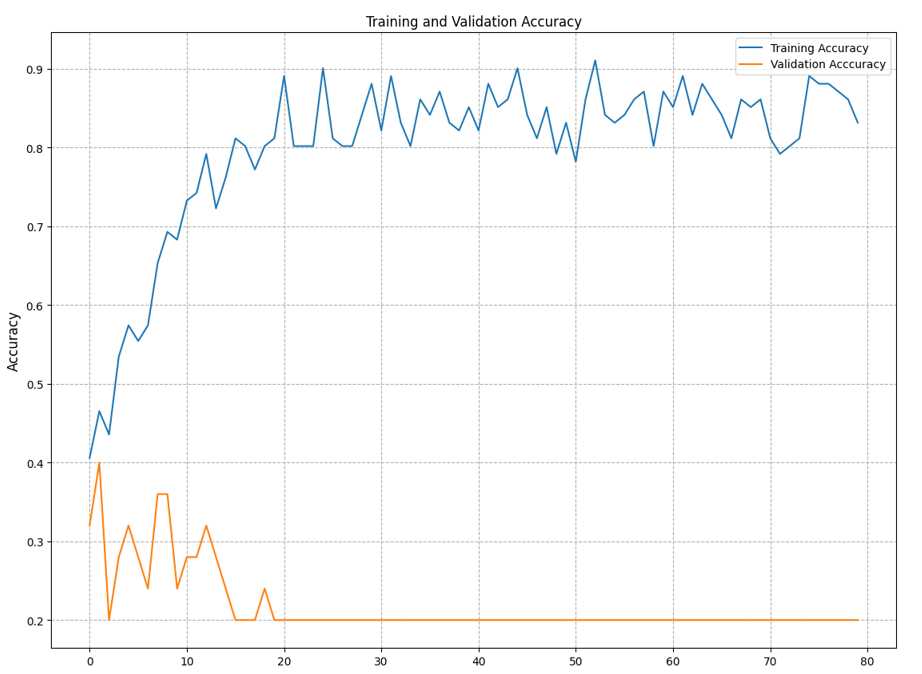
\includegraphics[scale=0.6]{gambar/AccIndRNNnoAug.png}
  % Keterangan gambar yang diinputkan
  \caption{Akurasi IndRNN Tanpa Data Augmentasi}
  % Label referensi dari gambar yang diinputkan
  \label{fig:AccIndRNNnoaug}
\end{figure}

\begin{figure} [H] \centering
  % Nama dari file gambar yang diinputkan
  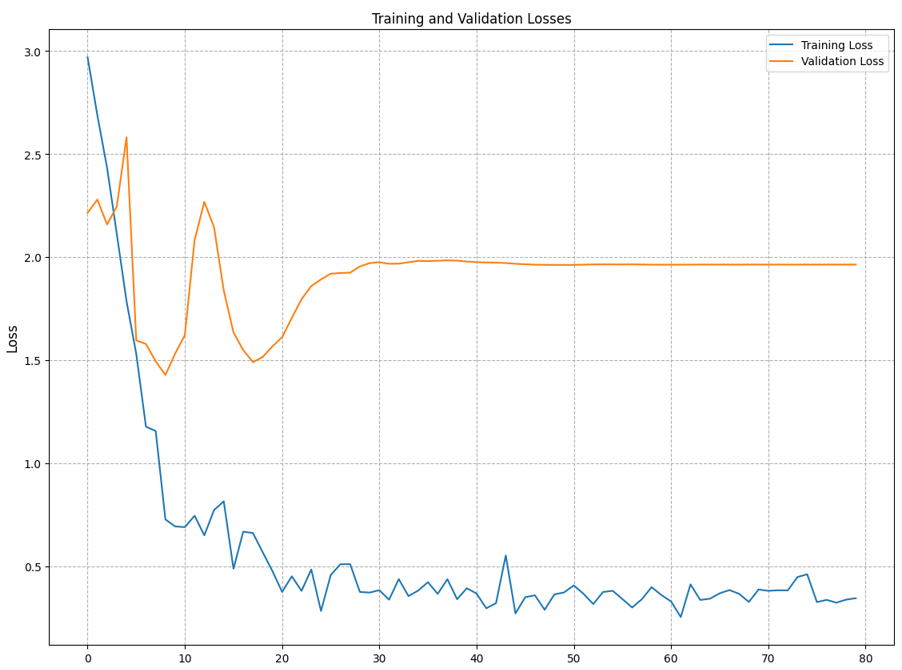
\includegraphics[scale=0.6]{gambar/LossIndRNNnoAug.png}
  % Keterangan gambar yang diinputkan
  \caption{Loss IndRNN Tanpa Data Augmentasi}
  % Label referensi dari gambar yang diinputkan
  \label{fig:LossIndRNNnoaug}
\end{figure}

\newpage
Berikut merupakan gambar loss dan akurasi dari data training yang teraugmentasi dan
data validasi yang terbaik:
\begin{figure} [H] \centering
  % Nama dari file gambar yang diinputkan
  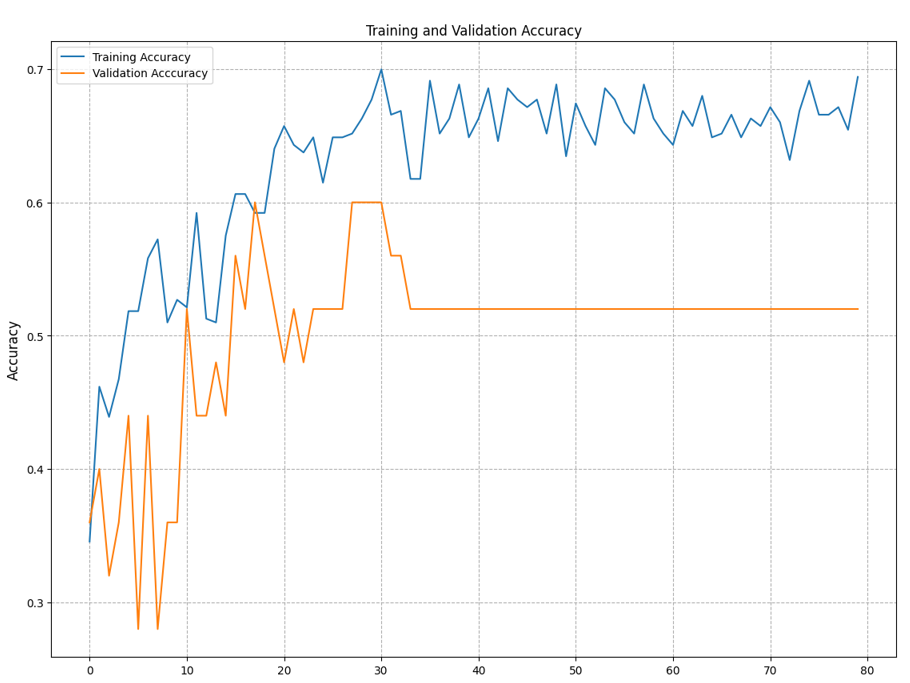
\includegraphics[scale=0.6]{gambar/AccIndRNNAug.png}
  % Keterangan gambar yang diinputkan
  \caption{Akurasi dan Loss IndRNN Dengan Data Augmentasi}
  % Label referensi dari gambar yang diinputkan
  \label{fig:AccIndRNNaug}
\end{figure}

\begin{figure} [H] \centering
  % Nama dari file gambar yang diinputkan
  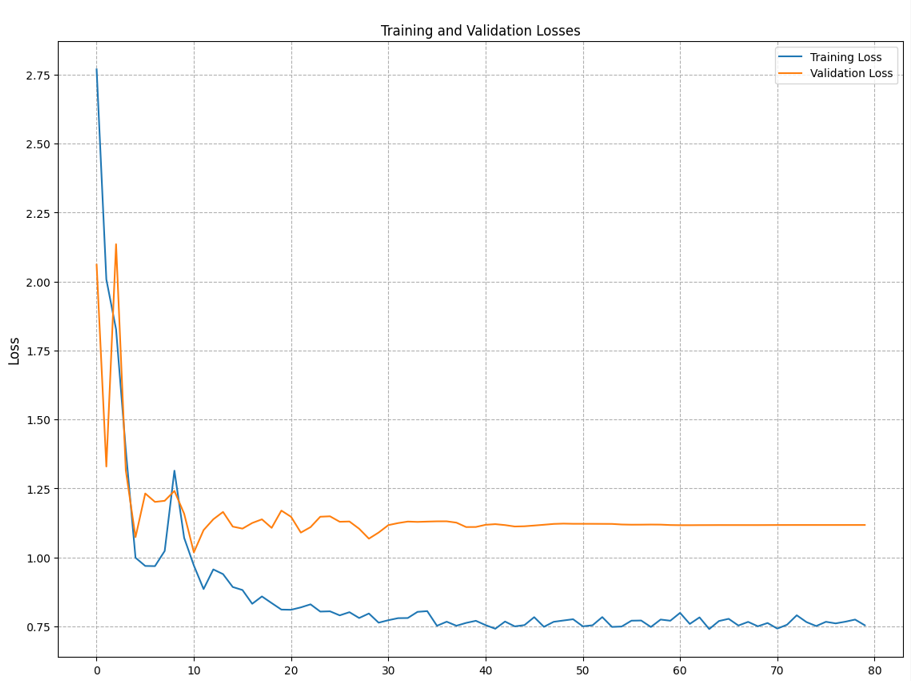
\includegraphics[scale=0.6]{gambar/LossIndRNNAug.png}
  % Keterangan gambar yang diinputkan
  \caption{Akurasi dan Loss IndRNN Dengan Data Augmentasi}
  % Label referensi dari gambar yang diinputkan
  \label{fig:LossIndRNNaug}
\end{figure}

Data pada gambar \ref{fig:AccIndRNNnoaug} dan gambar \ref{fig:LossIndRNNnoaug} menunjukkan akurasi training
sebesar 0.8378 dan akurasi validasi sebesar 0.2 serta loss training sebesar 0.3236
dan loss validasi sebesar 1.9798 . Sedangkan data pada gambar \ref{fig:AccIndRNNaug} dan gambar \ref{fig:LossIndRNNaug}
menunjukkan akurasi training sebesar 0.6943 dan akurasi validasi sebesar 0.52 serta
loss training sebesar 0.7529 dan loss validasi sebesar 1.1258 .

\subsection{Long short term memory network}
Berikut merupakan gambar loss dan akurasi dari data training yang tidak teraugmentasi dan
data validasi yang terbaik:

\begin{figure} [H] \centering
  % Nama dari file gambar yang diinputkan
  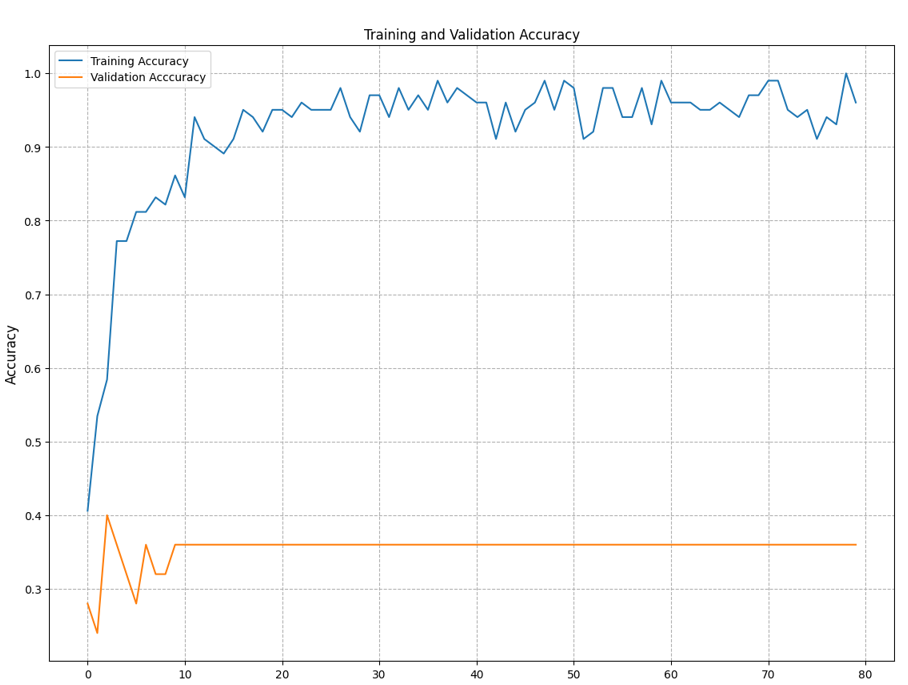
\includegraphics[scale=0.6]{gambar/AccLSTMnoAug.png}
  % Keterangan gambar yang diinputkan
  \caption{Akurasi dan Loss LSTM Tanpa Data Augmentasi}
  % Label referensi dari gambar yang diinputkan
  \label{fig:AccLSTMnoaug}
\end{figure}

\begin{figure} [H] \centering
  % Nama dari file gambar yang diinputkan
  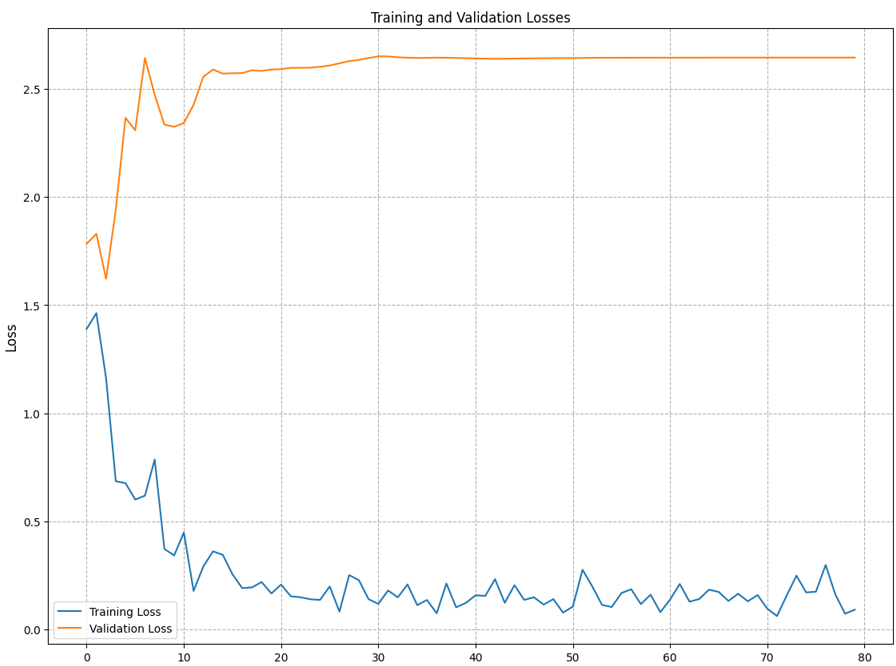
\includegraphics[scale=0.6]{gambar/LossLSTMnoAug.png}
  % Keterangan gambar yang diinputkan
  \caption{Akurasi dan Loss LSTM Tanpa Data Augmentasi}
  % Label referensi dari gambar yang diinputkan
  \label{fig:LossLSTMnoaug}
\end{figure}

\newpage
Berikut merupakan gambar loss dan akurasi dari data training yang teraugmentasi dan
data validasi yang terbaik:
\begin{figure} [H] \centering
  % Nama dari file gambar yang diinputkan
  \includegraphics[scale=0.6]{gambar/AccLSTMaug.png}
  % Keterangan gambar yang diinputkan
  \caption{Akurasi dan Loss LSTM Dengan Data Augmentasi}
  % Label referensi dari gambar yang diinputkan
  \label{fig:AccLSTMaug}
\end{figure}

\begin{figure} [H] \centering
  % Nama dari file gambar yang diinputkan
  \includegraphics[scale=0.6]{gambar/LossLSTMaug.png}
  % Keterangan gambar yang diinputkan
  \caption{Akurasi dan Loss LSTM Dengan Data Augmentasi}
  % Label referensi dari gambar yang diinputkan
  \label{fig:LossLSTMaug}
\end{figure}

Data pada gambar \ref{fig:AccLSTMnoaug} dan gambar \ref{fig:LossLSTMnoaug} menunjukkan akurasi training sebesar 0.9732
dan akurasi validasi sebesar 0.32 serta loss training sebesar 0.1342 dan loss validasi
sebesar 2.4947 . Sedangkan data pada gambar \ref{fig:AccLSTMaug} dan gambar \ref{fig:LossLSTMaug}
menunjukkan akurasi training sebesar 0.9354 dan akurasi validasi sebesar 0.4
serta loss training sebesar 0.3541 dan loss validasi sebesar 1.7487 .

\section{Hasil Evaluasi Model}
Hasil evaluasi yang dihasilkan pada penelitian ini berbentuk:
\begin{enumerate}[nolistsep]
  \item Confusion Matrix

        Confusion matrix adalah tabel yang menunjukkan jumlah prediksi yang benar dan salah yang dilakukan oleh
        model. Confusion matrix terdiri dari empat komponen: \emph{true positive} (TP), \emph{true negative} (TN), \emph{false
        positive} (FP), dan \emph{false negative} (FN). Dengan menggunakan confusion matrix, kita dapat menghitung
        metrik evaluasi lainnya.

  \item Akurasi

        Akurasi mengukur persentase prediksi yang benar secara keseluruhan. Ini dihitung dengan membagi jumlah
        prediksi yang benar (TP dan TN) dengan total sampel dalam dataset. Akurasi dapat memberikan gambaran
        umum tentang sejauh mana model dapat memprediksi dengan benar, tetapi dapat menghasilkan hasil yang
        bias jika terdapat ketimpangan jumlah sampel pada setiap kelas

  \item Presisi

        Presisi mengukur persentase prediksi positif yang benar. Ini mengukur sejauh mana prediksi positif
        model adalah akurat. Presisi dihitung dengan membagi TP dengan jumlah prediksi positif (TP dan FP).

  \item Recall

        Recall, juga dikenal sebagai \emph{Sensitivity} atau \emph{True Positive Rate} (TPR), mengukur persentase sampel
        positif yang diprediksi dengan benar. Ini mengukur sejauh mana model dapat menemukan semua sampel
        positif yang sebenarnya. Recall dihitung dengan membagi TP dengan jumlah sampel positif (TP dan FN).

  \item F1-Score

        F1-Score adalah penggabungan presisi dan recall menjadi satu metrik yang mencerminkan keseimbangan
        antara keduanya. F1-Score dihitung sebagai rata-rata harmonis dari presisi dan recall, dan memberikan
        gambaran keseluruhan tentang performa model. F1-Score berguna ketika kelas target memiliki
        ketidakseimbangan jumlah sampel.

\end{enumerate}

\subsection{Independent Recurrent Neural Network}

Berikut merupakan gambar hasil evaluasi model IndRNN tanpa data augmentasi:
\newpage
\begin{figure} [H] \centering
  % Nama dari file gambar yang diinputkan
  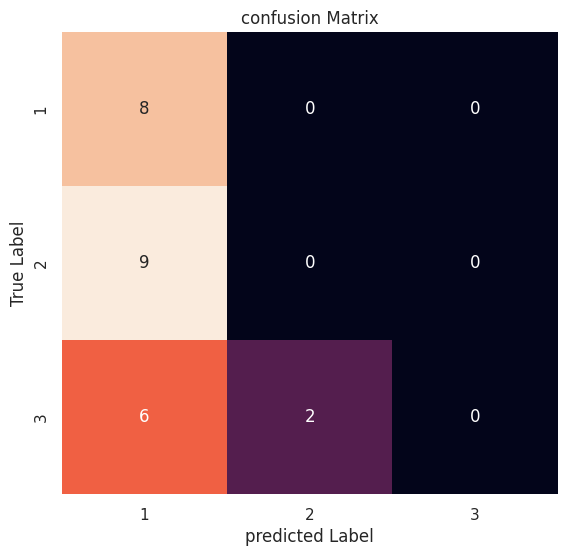
\includegraphics[scale=0.8]{gambar/CMIndRNNnoaug.png}
  % Keterangan gambar yang diinputkan
  \caption{Confusion Matrix IndRNN Tanpa Data Augmentasi}
  % Label referensi dari gambar yang diinputkan
  \label{fig:CMIndRNNnoaug}
\end{figure}

\begin{figure} [H] \centering
  % Nama dari file gambar yang diinputkan
  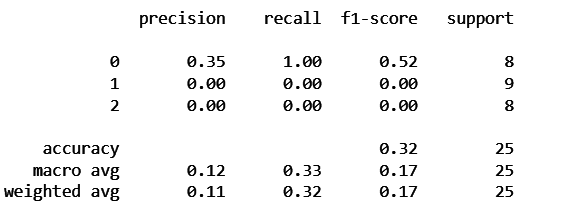
\includegraphics[scale=0.95]{gambar/scoreIndRNNnoaug.png}
  % Keterangan gambar yang diinputkan
  \caption{Evaluasi IndRNN Tanpa Data Augmentasi}
  % Label referensi dari gambar yang diinputkan
  \label{fig:ScoreIndRNNnoaug}
\end{figure}

Data yang didapatkan dari confusion matrix \ref{fig:CMIndRNNnoaug} didapatkan 8 video yang bernilai benar
dengan hasil akurasi sebesar 0.32, hasil nilai presisi model pada kelas 1 sebesar 0.35, hasil nilai
presisi model pada kelas 2 sebesar 0.0, hasil nilai presisi model pada kelas 3 sebesar 0.0. Model menghasilkan
nilai recall sebesar 1.0 pada kelas 1, 0.0 pada kelas 2, dan 0.0 pada kelas 3. Nilai f1-score yang dihasilkan
oleh model sebesar 0.52 pada kelas 1, 0.0 pada kelas 2, 0.0 pada kelas 3.

Berikut merupakan gambar hasil evaluasi model IndRNN  dengan data augmentasi:
\newpage
\begin{figure} [H] \centering
  % Nama dari file gambar yang diinputkan
  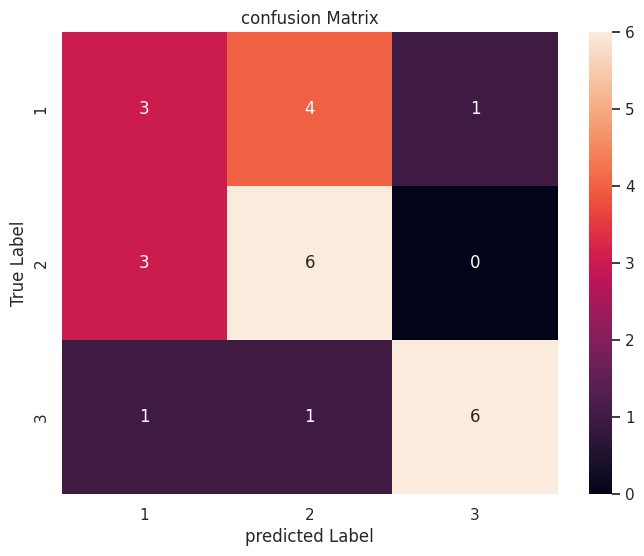
\includegraphics[scale=0.5]{gambar/CMIndRNNaug.png}
  % Keterangan gambar yang diinputkan
  \caption{Confusion Matrix IndRNN Dengan Data Augmentasi}
  % Label referensi dari gambar yang diinputkan
  \label{fig:CMIndRNNaug}
\end{figure}

\begin{figure} [H] \centering
  % Nama dari file gambar yang diinputkan
  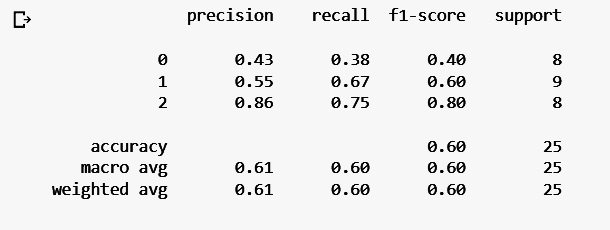
\includegraphics[scale=0.85]{gambar/scoreIndRNNaug.png}
  % Keterangan gambar yang diinputkan
  \caption{Evaluasi IndRNN Dengan Data Augmentasi}
  % Label referensi dari gambar yang diinputkan
  \label{fig:ScoreIndRNNaug}
\end{figure}

Data yang didapatkan dari confusion matrix \ref{fig:CMIndRNNaug} didapatkan 15 video yang bernilai benar
dengan hasil akurasi sebesar 0.6, hasil nilai presisi model pada kelas 1 sebesar 0.43, hasil nilai
presisi model pada kelas 2 sebesar 0.55, hasil nilai presisi model pada kelas 3 sebesar 0.86. Model menghasilkan
nilai recall sebesar 0.38 pada kelas 1, 0.67 pada kelas 2, dan 0.75 pada kelas 3. Nilai f1-score yang dihasilkan
oleh model sebesar 0.40 pada kelas 1, 0.60 pada kelas 2, 0.80 pada kelas 3.

\subsection{Long short term memory network}

Berikut merupakan gambar hasil evaluasi model LSTM tanpa data augmentasi:
\newpage
\begin{figure} [H] \centering
  % Nama dari file gambar yang diinputkan
  \includegraphics[scale=0.7]{gambar/CMLSTMnoAug.png}
  % Keterangan gambar yang diinputkan
  \caption{Akurasi dan Loss LSTM Tanpa Data Augmentasi}
  % Label referensi dari gambar yang diinputkan
  \label{fig:CMLSTMnoaug}
\end{figure}

\begin{figure} [H] \centering
  % Nama dari file gambar yang diinputkan
  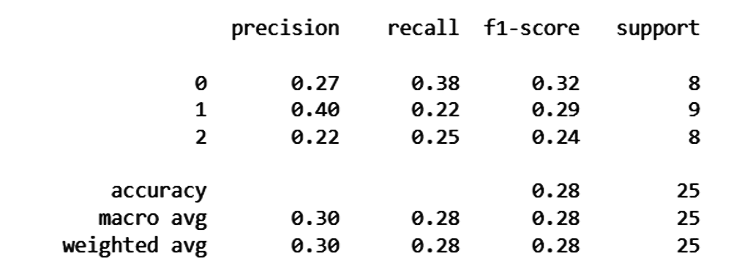
\includegraphics[scale=0.85]{gambar/scoreLSTMnoaug.png}
  % Keterangan gambar yang diinputkan
  \caption{Evaluasi LSTM Dengan Data Augmentasi}
  % Label referensi dari gambar yang diinputkan
  \label{fig:ScoreLSTMnoaug}
\end{figure}
Data yang didapatkan dari confusion matrix \ref{fig:CMLSTMnoaug} didapatkan 7 video yang bernilai benar
dengan hasil akurasi sebesar 0.28, hasil nilai presisi model pada kelas 1 sebesar 0.27, hasil nilai
presisi model pada kelas 2 sebesar 0.4, hasil nilai presisi model pada kelas 3 sebesar 0.22. Model menghasilkan
nilai recall sebesar 0.38 pada kelas 1, 0.22 pada kelas 2, dan 0.25 pada kelas 3. Nilai f1-score yang dihasilkan
oleh model sebesar 0.32 pada kelas 1, 0.29 pada kelas 2, 0.24 pada kelas 3.

Berikut merupakan gambar hasil evaluasi model LSTM dengan data augmentasi:
\begin{figure} [H] \centering
  % Nama dari file gambar yang diinputkan
  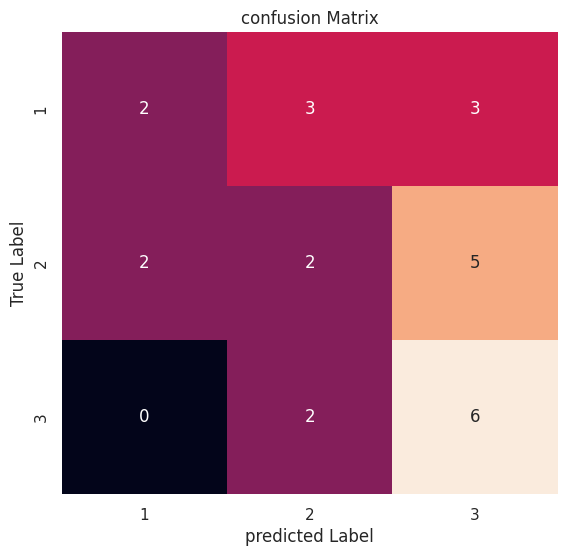
\includegraphics[scale=0.45]{gambar/CMLSTMaug.png}
  % Keterangan gambar yang diinputkan
  \caption{Confusion Matrix LSTM Dengan Data Augmentasi}
  % Label referensi dari gambar yang diinputkan
  \label{fig:CMLSTMaug}
\end{figure}

\begin{figure} [H] \centering
  % Nama dari file gambar yang diinputkan
  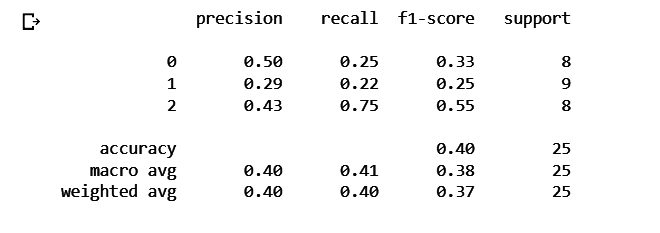
\includegraphics[scale=0.75]{gambar/scoreLSTMaug.png}
  % Keterangan gambar yang diinputkan
  \caption{Evaluasi LSTM Dengan Data Augmentasi}
  % Label referensi dari gambar yang diinputkan
  \label{fig:ScoreLSTMaug}
\end{figure}
Data yang didapatkan dari confusion matrix \ref{fig:CMLSTMaug} didapatkan 10 video yang bernilai benar
dengan hasil akurasi sebesar 0.40, hasil nilai presisi model pada kelas 1 sebesar 0.5, hasil nilai
presisi model pada kelas 2 sebesar 0.29, hasil nilai presisi model pada kelas 3 sebesar 0.43. Model menghasilkan
nilai recall sebesar 0.25 pada kelas 1, 0.22 pada kelas 2, dan 0.275 pada kelas 3. Nilai f1-score yang dihasilkan
oleh model sebesar 0.33 pada kelas 1, 0.25 pada kelas 2, 0.55 pada kelas 3.

\subsection{Support Vector Machine}
Berikut merupakan gambar hasil evaluasi model SVM tanpa data augmentasi:

\newpage
\begin{figure} [H] \centering
  % Nama dari file gambar yang diinputkan
  \includegraphics[scale=5]{gambar/CMSVMnoAug.png}
  % Keterangan gambar yang diinputkan
  \caption{Akurasi dan Loss SVM Tanpa Data Augmentasi}
  % Label referensi dari gambar yang diinputkan
  \label{fig:CMSVMnoaug}
\end{figure}

\begin{figure} [H] \centering
  % Nama dari file gambar yang diinputkan
  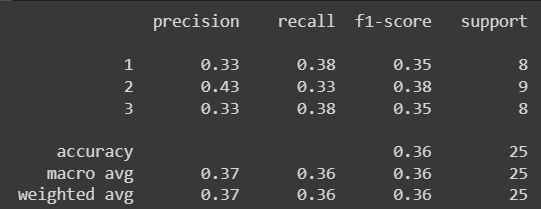
\includegraphics[scale=1]{gambar/scoreSVMnoaug.png}
  % Keterangan gambar yang diinputkan
  \caption{Evaluasi SVM Dengan Data Augmentasi}
  % Label referensi dari gambar yang diinputkan
  \label{fig:ScoreSVMnoaug}
\end{figure}

Data yang didapatkan dari confusion matrix 4.17 didapatkan 9 video yang bernilai benar
dengan hasil akurasi sebesar 0.36, hasil nilai presisi model pada kelas 1 sebesar 0.33, hasil
nilai presisi model pada kelas 2 sebesar 0.43, hasil nilai presisi model pada kelas 3 sebesar 0.33.
Model menghasilkan nilai recall sebesar 0.38 pada kelas 1, 0.33 pada kelas 2, dan 0.38 pada
kelas 3. Nilai f1-score yang dihasilkan oleh model sebesar 0.35 pada kelas 1, 0.38 pada kelas
2, 0.35 pada kelas 3.

Berikut merupakan gambar hasil evaluasi model SVM dengan data augmentasi:

\begin{figure} [H] \centering
  % Nama dari file gambar yang diinputkan
  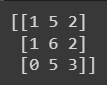
\includegraphics[scale=5]{gambar/CMSVMaug.png}
  % Keterangan gambar yang diinputkan
  \caption{Confusion Matrix SVM Dengan Data Augmentasi}
  % Label referensi dari gambar yang diinputkan
  \label{fig:CMSVMaug}
\end{figure}

\begin{figure} [H] \centering
  % Nama dari file gambar yang diinputkan
  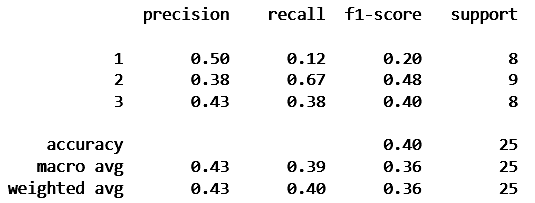
\includegraphics[scale=1]{gambar/scoreSVMaug.png}
  % Keterangan gambar yang diinputkan
  \caption{Evaluasi SVM Dengan Data Augmentasi}
  % Label referensi dari gambar yang diinputkan
  \label{fig:ScoreSVMaug}
\end{figure}

Data yang didapatkan dari confusion matrix 4.19 didapatkan 10 video yang bernilai benar
dengan hasil akurasi sebesar 0.40, hasil nilai presisi model pada kelas 1 sebesar 0.50, hasil
nilai presisi model pada kelas 2 sebesar 0.38, hasil nilai presisi model pada kelas 3 sebesar 0.43.
Model menghasilkan nilai recall sebesar 0.12 pada kelas 1, 0.67 pada kelas 2, dan 0.38 pada
kelas 3. Nilai f1-score yang dihasilkan oleh model sebesar 0.20 pada kelas 1, 0.48 pada kelas
2, 0.40 pada kelas 3.

\section{Hasil Testing Model}
\subsection{Independent Recurrent Neural Network}

Berikut merupakan gambar hasil evaluasi model IndRNN tanpa data augmentasi:
\newpage
\begin{figure} [H] \centering
  % Nama dari file gambar yang diinputkan
  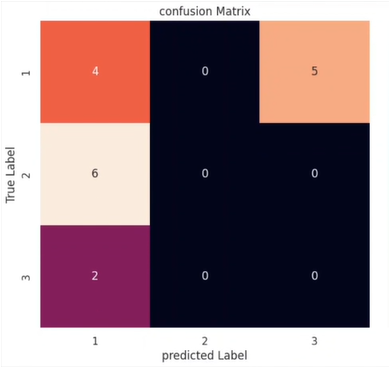
\includegraphics[scale=1.3]{gambar/CMIndRNNnoaug2.png}
  % Keterangan gambar yang diinputkan
  \caption{Confusion Matrix IndRNN Tanpa Data Augmentasi}
  % Label referensi dari gambar yang diinputkan
  \label{fig:CMIndRNNnoaug2}
\end{figure}

\begin{figure} [H] \centering
  % Nama dari file gambar yang diinputkan
  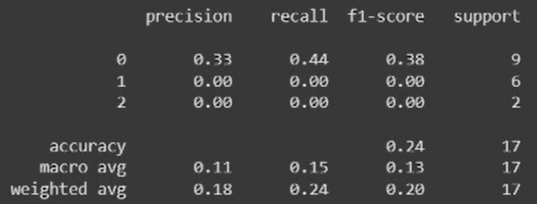
\includegraphics[scale=1]{gambar/scoreIndRNNnoaug2.png}
  % Keterangan gambar yang diinputkan
  \caption{Testing IndRNN Tanpa Data Augmentasi}
  % Label referensi dari gambar yang diinputkan
  \label{fig:ScoreIndRNNnoaug2}
\end{figure}

Data yang didapatkan dari confusion matrix \ref{fig:CMIndRNNnoaug2} didapatkan 4 video yang bernilai benar
dengan hasil akurasi sebesar 0.24, hasil nilai presisi model pada kelas 1 sebesar 0.33, hasil nilai
presisi model pada kelas 2 sebesar 0.0, hasil nilai presisi model pada kelas 3 sebesar 0.0. Model menghasilkan
nilai recall sebesar 0.44 pada kelas 1, 0.0 pada kelas 2, dan 0.0 pada kelas 3. Nilai f1-score yang dihasilkan
oleh model sebesar 0.38 pada kelas 1, 0.0 pada kelas 2, 0.0 pada kelas 3.

Berikut merupakan gambar hasil evaluasi model IndRNN  dengan data augmentasi:
\newpage
\begin{figure} [H] \centering
  % Nama dari file gambar yang diinputkan
  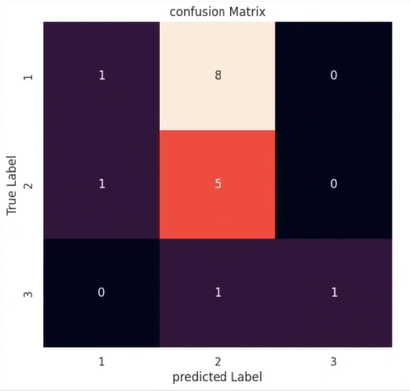
\includegraphics[scale=1.3]{gambar/CMIndRNNaug2.png}
  % Keterangan gambar yang diinputkan
  \caption{Confusion Matrix IndRNN Dengan Data Augmentasi}
  % Label referensi dari gambar yang diinputkan
  \label{fig:CMIndRNNaug2}
\end{figure}

\begin{figure} [H] \centering
  % Nama dari file gambar yang diinputkan
  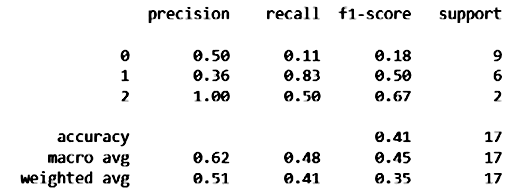
\includegraphics[scale=1]{gambar/scoreIndRNNaug2.png}
  % Keterangan gambar yang diinputkan
  \caption{Testing IndRNN Dengan Data Augmentasi}
  % Label referensi dari gambar yang diinputkan
  \label{fig:ScoreIndRNNaug}
\end{figure}

Data yang didapatkan dari confusion matrix \ref{fig:CMIndRNNaug2} didapatkan 7 video yang bernilai benar
dengan hasil akurasi sebesar 0.41, hasil nilai presisi model pada kelas 1 sebesar 0.50, hasil nilai
presisi model pada kelas 2 sebesar 0.36, hasil nilai presisi model pada kelas 3 sebesar 1.0. Model menghasilkan
nilai recall sebesar 0.11 pada kelas 1, 0.83 pada kelas 2, dan 0.50 pada kelas 3. Nilai f1-score yang dihasilkan
oleh model sebesar 0.18 pada kelas 1, 0.50 pada kelas 2, 0.67 pada kelas 3.

\subsection{Long short term memory network}

Berikut merupakan gambar hasil evaluasi model LSTM tanpa data augmentasi:
\newpage
\begin{figure} [H] \centering
  % Nama dari file gambar yang diinputkan
  \includegraphics[scale=1.3]{gambar/CMLSTMnoAug2.png}
  % Keterangan gambar yang diinputkan
  \caption{Confusion Matrix LSTM Tanpa Data Augmentasi}
  % Label referensi dari gambar yang diinputkan
  \label{fig:CMLSTMnoaug2}
\end{figure}

\begin{figure} [H] \centering
  % Nama dari file gambar yang diinputkan
  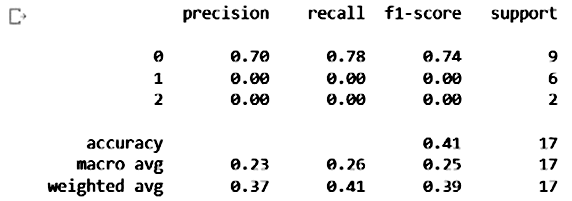
\includegraphics[scale=1]{gambar/scoreLSTMnoaug2.png}
  % Keterangan gambar yang diinputkan
  \caption{Testing LSTM Dengan Data Augmentasi}
  % Label referensi dari gambar yang diinputkan
  \label{fig:ScoreLSTMnoaug2}
\end{figure}
Data yang didapatkan dari confusion matrix \ref{fig:CMLSTMnoaug2} didapatkan 7 video yang bernilai benar
dengan hasil akurasi sebesar 0.41, hasil nilai presisi model pada kelas 1 sebesar 0.70, hasil nilai
presisi model pada kelas 2 sebesar 0.0, hasil nilai presisi model pada kelas 3 sebesar 0.0. Model menghasilkan
nilai recall sebesar 0.78 pada kelas 1, 0.0 pada kelas 2, dan 0.0 pada kelas 3. Nilai f1-score yang dihasilkan
oleh model sebesar 0.74 pada kelas 1, 0.0 pada kelas 2, 0.0 pada kelas 3.

Berikut merupakan gambar hasil evaluasi model LSTM dengan data augmentasi:
\begin{figure} [H] \centering
  % Nama dari file gambar yang diinputkan
  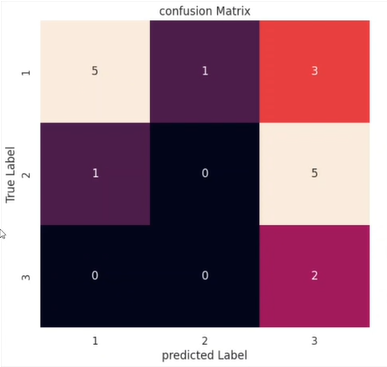
\includegraphics[scale=1.3]{gambar/CMLSTMaug2.png}
  % Keterangan gambar yang diinputkan
  \caption{Confusion Matrix LSTM Dengan Data Augmentasi}
  % Label referensi dari gambar yang diinputkan
  \label{fig:CMLSTMaug2}
\end{figure}

\begin{figure} [H] \centering
  % Nama dari file gambar yang diinputkan
  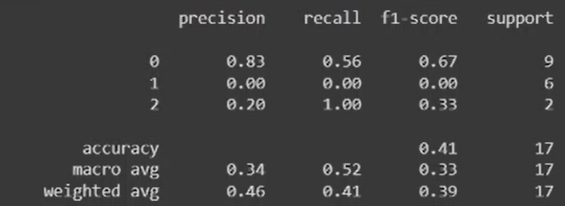
\includegraphics[scale=1]{gambar/scoreLSTMaug2.png}
  % Keterangan gambar yang diinputkan
  \caption{Testing LSTM Dengan Data Augmentasi}
  % Label referensi dari gambar yang diinputkan
  \label{fig:ScoreLSTMaug2}
\end{figure}
Data yang didapatkan dari confusion matrix \ref{fig:CMLSTMaug2} didapatkan 7 video yang bernilai benar
dengan hasil akurasi sebesar 0.41, hasil nilai presisi model pada kelas 1 sebesar 0.83, hasil nilai
presisi model pada kelas 2 sebesar 0.0, hasil nilai presisi model pada kelas 3 sebesar 0.20. Model menghasilkan
nilai recall sebesar 0.56 pada kelas 1, 0.0 pada kelas 2, dan 1.0 pada kelas 3. Nilai f1-score yang dihasilkan
oleh model sebesar 0.67 pada kelas 1, 0.0 pada kelas 2, 0.33 pada kelas 3.

\subsection{Support Vector Machine}
Berikut merupakan gambar hasil evaluasi model SVM tanpa data augmentasi:

\newpage
\begin{figure} [H] \centering
  % Nama dari file gambar yang diinputkan
  \includegraphics[scale=5]{gambar/CMSVMnoAug2.png}
  % Keterangan gambar yang diinputkan
  \caption{Confusion Matrix SVM Tanpa Data Augmentasi}
  % Label referensi dari gambar yang diinputkan
  \label{fig:CMSVMnoaug2}
\end{figure}

\begin{figure} [H] \centering
  % Nama dari file gambar yang diinputkan
  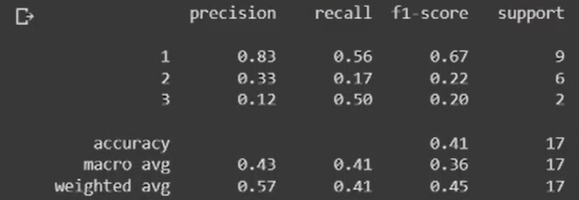
\includegraphics[scale=1]{gambar/scoreSVMnoaug2.png}
  % Keterangan gambar yang diinputkan
  \caption{Testing SVM Dengan Data Augmentasi}
  % Label referensi dari gambar yang diinputkan
  \label{fig:ScoreSVMnoaug2}
\end{figure}

Data yang didapatkan dari confusion matrix \ref{fig:CMSVMnoaug2} didapatkan 7 video yang bernilai benar
dengan hasil akurasi sebesar 0.41, hasil nilai presisi model pada kelas 1 sebesar 0.83, hasil
nilai presisi model pada kelas 2 sebesar 0.33, hasil nilai presisi model pada kelas 3 sebesar 0.12.
Model menghasilkan nilai recall sebesar 0.56 pada kelas 1, 0.17 pada kelas 2, dan 0.50 pada
kelas 3. Nilai f1-score yang dihasilkan oleh model sebesar 0.67 pada kelas 1, 0.22 pada kelas
2, 0.20 pada kelas 3.

Berikut merupakan gambar hasil evaluasi model SVM dengan data augmentasi:

\begin{figure} [H] \centering
  % Nama dari file gambar yang diinputkan
  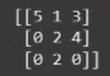
\includegraphics[scale=5]{gambar/CMSVMaug2.png}
  % Keterangan gambar yang diinputkan
  \caption{Confusion Matrix SVM Dengan Data Augmentasi}
  % Label referensi dari gambar yang diinputkan
  \label{fig:CMSVMaug2}
\end{figure}

\begin{figure} [H] \centering
  % Nama dari file gambar yang diinputkan
  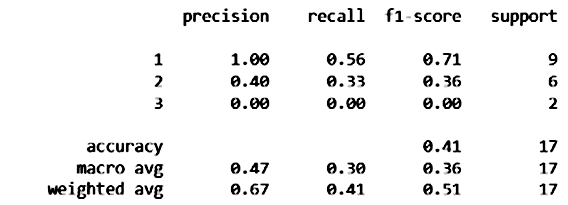
\includegraphics[scale=1]{gambar/scoreSVMaug2.png}
  % Keterangan gambar yang diinputkan
  \caption{Testing SVM Dengan Data Augmentasi}
  % Label referensi dari gambar yang diinputkan
  \label{fig:ScoreSVMaug2}
\end{figure}

Data yang didapatkan dari confusion matrix \ref{fig:CMSVMaug2} didapatkan 7 video yang bernilai benar
dengan hasil akurasi sebesar 0.41, hasil nilai presisi model pada kelas 1 sebesar 1.0, hasil
nilai presisi model pada kelas 2 sebesar 0.40, hasil nilai presisi model pada kelas 3 sebesar 0.0.
Model menghasilkan nilai recall sebesar 0.56 pada kelas 1, 0.33 pada kelas 2, dan 0.0 pada
kelas 3. Nilai f1-score yang dihasilkan oleh model sebesar 0.71 pada kelas 1, 0.36 pada kelas
2, 0.0 pada kelas 3.

\newpage
\section{Pembahasan}
\label{sec:analisispengujian}

Dari pengujian yang telah dilakukan, berdasarkan hasil training kedua model
yaitu dengan IndRNN dan LSTM didapatkan tabel sebagai berikut:

% Contoh pembuatan tabel
\begin{longtable}{|c|c|c|c|c|}
  \caption{Data Hasil Training Model}
  \label{tb:EnergiKecepatan}                                                                                            \\
  \hline
  \rowcolor[HTML]{C0C0C0}
  \textbf{Model}                & \textbf{Akurasi} & \textbf{Validasi} & \textbf{Loss Akurasi} & \textbf{Loss Validasi} \\
  \hline
  IndRNN tanpa data augmentasi  & 0.8378           & 0.2               & 0.3236                & 1.9798                 \\
  IndRNN dengan data augmentasi & 0.6943           & 0.52              & 0.7529                & 1.1258                 \\
  LSTM tanpa data augmentasi    & 0.9732           & 0.32              & 0.1342                & 2.4947                 \\
  LSTM dengan data augmentasi   & 0.9354           & 0.4               & 0.3541                & 1.7487                 \\
  \hline
\end{longtable}

\begin{longtable}{|c|c|}
  \caption{Data Hasil Evaluasi Model}
  \label{tb:EnergiKecepatan}                                \\
  \hline
  \rowcolor[HTML]{C0C0C0}
  \textbf{Model}                & \textbf{Confusion Matrix} \\
  \hline
  IndRNN tanpa data augmentasi  & 8 data benar              \\
  IndRNN dengan data augmentasi & 15 data benar             \\
  LSTM tanpa data augmentasi    & 7 data benar              \\
  LSTM dengan data augmentasi   & 10 data benar             \\
  SVM tanpa data augmentasi     & 9 data benar              \\
  SVM dengan data augmentasi    & 10 data benar             \\
  \hline
\end{longtable}

Model yang pertama yaitu IndRNN dengan input (x) berupa nilai EAR serta MAR dan kelas
sebagai target (y) mendapatkan hasil training yang kurang baik dengan akurasi sebesar 0.8378 dan validasi akurasi sebesar 0.2,
pada grafik terlihat model mengalami overfitting.

Model yang kedua yaitu IndRNN dengan input (x) berupa nilai EAR serta MAR yang teraugmentasi dan kelas
sebagai target (y) mendapatkan hasil training yang paling baik diantara model lainnya karena tidak mengalami
overfitting dengan akurasi 0.6943 dan validasi akurasi 0.52.

Model yang ketiga yaitu LSTM dengan input (x) berupa nilai EAR serta MAR dan kelas
sebagai target (y) mendapatkan hasil training yang kurang baik dengan akurasi sebesar 0.9732 dan validasi akurasi sebesar 0.32
, pada grafik terlihat model mengalami overfitting.

Model yang keempat yaitu LSTM dengan input (x) berupa nilai EAR serta MAR yang teraugmentasi dan kelas
sebagai target (y) mendapatkan hasil training yang lebih baik daripada LSTM dengan data yang tidak teraugmentasi,
selain itu pada grafik juga terlihat model mengalami overfitting dengan akurasi 0.9354 dan validasi akurasi 0.4.

Model yang kelima yaitu SVM dengan input (x) berupa nilai EAR serta MAR dan kelas
sebagai target (y) mendapatkan hasil evaluasi yang lebih baik jika dibandingkan dengan IndRNN dan LSTM tanpa data
augmentasi yang menghasilkan 9 nilai benar.

Model yang keenam yaitu SVM dengan input (x) berupa nilai EAR serta MAR yang teraugmentasi dan kelas sebagai target 
(y) mendapatkan hasil evaluasi yang lebih baik dari SVM dengan data yang tidak teraugmentasi dengan jumlah 10 nilai benar. 

Berdasarkan keseluruhan hasil training dan evaluasi, didapatkan bahwa model klasifikasi terbaik yaitu model IndRNN yang
ditraining menggunakan data yang telah diaugmentasi. Hal ini memvalidasi bahwa model IndRNN pada klasifikasi kantuk
lebih baik daripada menggunakan SVM dan LSTM.

\cleardoublepage

% Bab 5 penutup
\chapter{KESIMPULAN DAN SARAN}
\label{chap:penutup}

% Ubah bagian-bagian berikut dengan isi dari penutup
Bab ini menjelaskan mengenai kesimpulan yang telah didapat dari proses penelitian
tugas akhir.

\section{Kesimpulan}
\label{sec:kesimpulan}

Pada Tugas Akhir ini telah dijelaskan pengembangan Sistem Klasifikasi Kantuk Berdasarkan
Pola Kedipan Mata dan Pola Bukaan Mulut dengan IndRNN. Dari hasil pengujian yang telah
dilakukan pada bab sebelumnya model klasifikasi kantuk IndRNN tanpa data training yang diaugmentasi
menghasilkan akurasi sebesar 0.8378 dan akurasi validasi sebesar 0.2. Sedangkan model klasifikasi
kantuk IndRNN yang menggunakan data training teraugmentasi menghasilkan akurasi sebesar 0.6943
dan akurasi validasi sebesar 0.52, lebih baik jika dibandingkan dengan kedua model yang lainnya karena
cenderung tidak overfitting. Kedua model lain yang dibuat adalah model LSTM tanpa data training 
yang diaugmentasi menghasilkan akurasi sebesar 0.9732 dan akurasi validasi sebesar 0.32 dan model 
klasifikasi kantuk LSTM yang menggunakan data training teraugmentasi yang menghasilkan akurasi 
sebesar 0.9354 dan akurasi validasi sebesar 0.4 serta model SVM tanpa data training yang
diaugmentasi menghasilkan akurasi sebesar 0.36 pada evaluasi model dan model 
SVM yang menggunakan data training teraugmentasi menghasilkan akurasi sebesar 
0.40 pada evaluasi model.

Berdasarkan keseluruhan hasil evaluasi, didapatkan bahwa model klasifikasi
terbaik yaitu model IndRNN yang ditraining menggunakan data yang telah diaugmentasi
dengan menghasilkan 15 data benar jika dibandingkan dengan model LSTM dan SVM yang menghasilkan
10 data benar.


% \begin{enumerate}[nolistsep]
%       \item IndRNN dapat diimplementasikan untuk membuat model klasifikasi kantuk dengan
%             model LSTM dan SVM yang digunakan sebagai pembanding kinerja IndRNN.

%       \item Model klasifikasi kantuk menggunakan IndRNN tanpa data training yang
%             diaugmentasi menghasilkan akurasi sebesar 0.8378 dan akurasi validasi sebesar 0.2.
%             Sedangkan model klasifikasi kantuk IndRNN yang menggunakan data training teraugmentasi
%             menghasilkan akurasi sebesar 0.6943 dan akurasi validasi sebesar 0.52.

%       \item Model klasifikasi kantuk menggunakan LSTM tanpa data training yang
%             diaugmentasi menghasilkan akurasi sebesar 0.9732 dan akurasi validasi sebesar 0.32.
%             Sedangkan model klasifikasi kantuk LSTM yang menggunakan data training teraugmentasi
%             menghasilkan akurasi sebesar 0.9354 dan akurasi validasi sebesar 0.4.

%       \item Model klasifikasi kantuk menggunakan SVM tanpa data training yang
%             diaugmentasi menghasilkan akurasi sebesar 0.36 pada evaluasi model.
%             Sedangkan model klasifikasi kantuk IndRNN yang menggunakan data training teraugmentasi
%             menghasilkan akurasi sebesar 0.40 pada evaluasi model.

%       \item Berdasarkan keseluruhan hasil evaluasi, didapatkan bahwa model klasifikasi
%             terbaik yaitu model IndRNN yang ditraining menggunakan data yang telah diaugmentasi
%             dengan menghasilkan 15 data benar jika dibandingkan dengan model LSTM dan SVM yang menghasilkan
%             10 data benar.

% \end{enumerate}

\section{Saran}
\label{chap:saran}

Untuk pengembangan lebih lanjut mengenai Tugas Akhir ini terdapat beberapa
kemungkinan perbaikan yang dapat dilakukan untuk penyempurnaan implementasi
model antara lain:

\begin{enumerate}[nolistsep]

      \item Mencoba model deteksi wajah yang berbeda karena saat menggunakan deteksi wajah dari library dlib
            didapati beberapa titik pada wajah tidak sesuai.

      \item Melakukan metode preprocessing yang berbeda untuk menghasilkan data yang lebih baik.

      \item Mencoba menggunakan hyperparameter yang berbeda, melakukan pengaturan training yang berbeda seperti
            jumlah epoch, learning rate, serta menggunakan fungsi callback yang berbeda.

\end{enumerate}

\cleardoublepage

\chapter*{DAFTAR PUSTAKA}
\addcontentsline{toc}{chapter}{DAFTAR PUSTAKA}
\renewcommand\refname{}
\vspace{2ex}
\renewcommand{\bibname}{}
\begingroup
\def\chapter*#1{}
\printbibliography
\endgroup
\cleardoublepage

% Lampiran
\begin{center}
    \Large
    \textbf{LAMPIRAN}
\end{center}


\addcontentsline{toc}{chapter}{LAMPIRAN}

\vspace{2ex}

\textbf{Lampiran A : Lampiran Program Preprocessing Data}

A.1 Fungsi Menghitung Nilai EAR
\begin{lstlisting}[language=Python]
    def calculate_EAR(eye):
    A = dist.euclidean(eye[1], eye[5])
    B = dist.euclidean(eye[2], eye[4])
    C = dist.euclidean(eye[0], eye[3])

    eye_aspect_ratio = (A + B) / (2.0 * C)

    return eye_aspect_ratio
\end{lstlisting}

A.2 Fungsi Menghitung Nilai MAR
\begin{lstlisting}[language=Python]
    V = dist.euclidean(mouth[1], mouth[7])
    W = dist.euclidean(mouth[2], mouth[6])
    X = dist.euclidean(mouth[3], mouth[5])
    Y = (V+W+X)/ 3.0

    Z =dist.euclidean(mouth[0], mouth[4])

    mouth_aspect_ratio = Y / Z

    if mouth_aspect_ratio < 0.001:
        mouth_aspect_ratio = 0.001
    return mouth_aspect_ratio
\end{lstlisting}

A.3 Program Interpolasi Data
\begin{lstlisting}[language=Python]
    for i in range (len(filenames)): #terahir index 
    data = pd.read_csv((inputNaN + filenames[i]), index_col=0, sep=',') 
    print(filenames[i])
    print(data.isnull().sum())
    for col in data.columns:
      # menghitung ear
      if col == 'ear_x' :
        left_ear = calc_ear(data[data.columns[1]], data[data.columns[2]], data[data.columns[3]], data[data.columns[4]],
                          data[data.columns[5]], data[data.columns[6]], data[data.columns[7]], data[data.columns[8]],
                          data[data.columns[9]], data[data.columns[10]], data[data.columns[11]], data[data.columns[12]])
        right_ear = calc_ear(data[data.columns[13]], data[data.columns[14]], data[data.columns[15]], data[data.columns[16]],
                          data[data.columns[17]], data[data.columns[18]], data[data.columns[19]], data[data.columns[20]],
                          data[data.columns[21]], data[data.columns[22]], data[data.columns[23]], data[data.columns[24]])
        value = pd.Series((left_ear+right_ear)/2)
      # menghitung mar
      elif col == 'mar_x':
        mar = calc_mar(data[data.columns[26]], data[data.columns[27]], data[data.columns[28]], data[data.columns[29]],
                          data[data.columns[30]], data[data.columns[31]], data[data.columns[32]], data[data.columns[33]],
                          data[data.columns[34]], data[data.columns[35]], data[data.columns[36]], data[data.columns[37]],
                          data[data.columns[38]], data[data.columns[39]], data[data.columns[40]], data[data.columns[41]])
        value = pd.Series(mar)
      else:
        value = data[col].interpolate() 
        value = round(value,0)
      data[col].fillna(value=value, inplace=True)
    filenames[i] = filenames[i].split(".")[0]
    data.to_csv('/mydrive/Output/' + filenames[i] + '.csv')
\end{lstlisting}

A.4 Fungsi Pemotongan Data
\begin{lstlisting}[language=Python]
    def begin_dat(data_num, data):
        slice_dat = data.iloc[:data_num]
        return slice_dat
  
    def last_dat(data_num, data):
        slice_dat = data.iloc[-data_num: ]
        return slice_dat
  
    def mid_dat(data_num, data):
        len_dat = len(data.iloc[:,0])
        mid = (len_dat - data_num) / 2
        slice_dat = data[ceil(mid):-floor(mid)]
        data.reset_index()
  
        return slice_dat
\end{lstlisting}

A.5 Program Labeling Data
\begin{lstlisting}[language=Python]
    for i in range (len(filenames)):
    data = pd.read_csv((output + filenames[i]), index_col=0, sep=',')
    data.reset_index(drop = True, inplace = True)
    df = data[['ear_x', 'mar_x']]
    slice_dat = mid_dat(16200, df)
    slice_dat.reset_index(drop = True, inplace = True)
    nama_file = filenames[i]
    label = label_name(nama_file)
    slice_dat['label'] = label
    print(slice_dat)
    filenames[i] = filenames[i].split(".")[0]
    slice_dat.to_csv('/mydrive/MarEar/' + filenames[i] + '.csv', index=False)
\end{lstlisting}

\newpage
A.6 Program Normalisasi Data
\begin{lstlisting}[language=Python]
    from sklearn.preprocessing import StandardScaler

    scaler = StandardScaler()
    arr = scaler.fit_transform(data[['ear_x', 'mar_x']])
    scaled_data = pd.DataFrame(arr, columns=['ear_x', 'mar_x'])
    scaled_data
\end{lstlisting}

A.7 Program Pembagian Data Training dan Data Validasi
\begin{lstlisting}[language=Python]
    def train_test_split(label, ratio):
    split_point = int(len(data[data.label == label])*ratio)
    return(data[data.label==label].iloc[:split_point,:], data[data.label==label].iloc[split_point:, :])

    split_ratio = (101/126)
    train_data = pd.DataFrame([])
    test_data = pd.DataFrame([])
    total_label = 3
    for i in range(total_label):
    (train, test) = train_test_split(i+1, split_ratio)
    train_data = pd.concat([train_data, train])
    test_data = pd.concat([test_data, test])
\end{lstlisting}

A.8 Program Sliding Window
\begin{lstlisting}[language=Python]
    WINDOW_LEN = 16200
    #step lebih kecil harus overlap dengan window_len
    STEP = 16199
    N_FEATURE = 2
    
    def generate_sequence(x, y, window_len, step):
      segments = []
      labels = []
      for i in range(0, len(x)-window_len, step):
        ear = x['ear_x'].values[i:i+window_len]
        mar = x['mar_x'].values[i:i+window_len]
        label = stats.mode(y['label'][i:i+window_len])[0][0]
        segments.append([ear, mar])
        labels.append(label)
    
      return segments, labels
\end{lstlisting}

\textbf{Lampiran B : Lampiran Program Training Data}
B.1 Fungsi Callback
\begin{lstlisting}[language=Python]
    # buat callbacks
    my_callbacks = [
        tf.keras.callbacks.ReduceLROnPlateau(factor=0.5, patience=5,),
        tf.keras.callbacks.ModelCheckpoint(filepath='/mydrive/TA/IndRNNaug_best.h5', save_best_only=True)]
\end{lstlisting}

B.2 Program Model IndRNN
\begin{lstlisting}[language=Python]
    def create_model():
    rnn2= Sequential()
    rnn2.add(Bidirectional(IndRNN(126, return_sequences=True, dropout=0.0, recurrent_dropout=0.0, kernel_initializer='orthogonal', kernel_regularizer=l2(L2), recurrent_regularizer=l2(L2),
            bias_regularizer=l2(L2),name="LSTM_1"), input_shape=(WINDOW_LEN, N_FEATURE)))
    rnn2.add(Dropout(0.3))
    rnn2.add(Flatten(name='Flatten'))
    rnn2.add(Dense(64, activation ='relu', name='Dense_3'))
    rnn2.add(Dropout(0.2))
    rnn2.add(Dense(32, activation ='relu', name='Dense_4'))
    rnn2.add(Dropout(0.1))
    rnn2.add(Dense(3, activation='softmax', kernel_regularizer=l2(L2), bias_regularizer=l2(L2)))
    rnn2.compile(optimizer=optimizers.Adam(0.000025), metrics=['accuracy'], loss='categorical_crossentropy')
    return rnn2
  
  model = create_model()
\end{lstlisting}

B.3 Program Model LSTM
\begin{lstlisting}[language=Python]
    lstm = Sequential()
    lstm.add(Bidirectional(LSTM(126, return_sequences=True,kernel_initializer='orthogonal', kernel_regularizer=l2(L2), recurrent_regularizer=l2(L2),
             bias_regularizer=l2(L2),name="LSTM_1"), input_shape=(WINDOW_LEN, N_FEATURE)))
    lstm.add(Dropout(0.3))
    lstm.add(Flatten(name='Flatten'))
    lstm.add(Dense(64, activation ='relu', name='Dense_3'))
    lstm.add(Dropout(0.2))
    lstm.add(Dense(32, activation ='relu', name='Dense_4'))
    lstm.add(Dropout(0.2))
    lstm.add(Dense(3, activation='softmax', kernel_regularizer=l2(L2), bias_regularizer=l2(L2)))
    lstm.compile(optimizer=optimizers.Adam(0.000025), metrics=['accuracy'], loss='categorical_crossentropy')
\end{lstlisting}

B.4 Program Model SVM
\begin{lstlisting}[language=Python]
    svm_model = svm.SVC(kernel='rbf')

    svm_model.fit(d2_train_dataset_x, ytrain)
\end{lstlisting}

\textbf{Lampiran C : Lampiran Program Evaluasi dan Testing Data}
\begin{lstlisting}[language=Python]
    import seaborn as sns
    from sklearn import metrics

    # Recreate the exact same model, including its weights and the optimizer
    new_model = tf.keras.models.load_model('/mydrive/TA/IndRNNaug_best.h5', custom_objects={'IndRNN':IndRNN})

    # Show the model architecture
    new_model.summary()

    y_pred_ohe = new_model.predict(x_test) #menghasilkan 3 kelas
    y_pred_ohe 

    y_pred_labels = np.argmax(y_pred_ohe, axis=1)
    y_pred_labels

    y_true_labels = np.argmax(y_test, axis=1)

    confusion_matrix = metrics.confusion_matrix(y_true= y_true_labels, y_pred= y_pred_labels)

    plt.figure(figsize=(8,6))
    sns.set(style='whitegrid')
    sns.heatmap(confusion_matrix, xticklabels=['1', '2', '3'], yticklabels=['1', '2', '3'], annot=True, fmt='d')
    plt.title("confusion Matrix")
    plt.ylabel("True Label")
    plt.xlabel("predicted Label")
    plt.show()

    from sklearn.metrics import classification_report
    print(classification_report(y_true_labels, y_pred_labels))
\end{lstlisting}

\cleardoublepage

% Biografi penulis
\begin{center}
  \Large
  \textbf{BIOGRAFI PENULIS}
\end{center}

\addcontentsline{toc}{chapter}{BIOGRAFI PENULIS}

\vspace{2ex}

\begin{wrapfigure}{L}{0.3\textwidth}
  \centering
  \vspace{-3ex}
  % Ubah file gambar berikut dengan file foto dari mahasiswa
  \includegraphics[width=0.3\textwidth]{gambar/formal.png}
  \vspace{-4ex}
\end{wrapfigure}

% Ubah kalimat berikut dengan biografi dari mahasiswa
\name{}, lahir di Gresik pada 2 November 2000. Penulis telah menempuh beberapa jenjang Pendidikan formal di 
beberapa sekolah yaitu: SMPN 2 Sidoarjo (2013-2016), dan SMAN 2 Sidoarjo (2016-2019). Penulis melanjutkan 
Pendidikan sarjana di Departemen Teknik Komputer Fakultas Teknologi Elektro dan Informatika Cerdas (FTEIC) 
Institut Teknologi Sepuluh Nopember (ITS) pada tahun 2019 yang terdaftar sebagai mahasiswa dengan nomor 
mahasiswa 07211940000017. Selama menjadi mahasiswa, penulis aktif mengikuti kegiatan kepanitiaan diantaranya Evolve,
MAGE 6, dan MAGE 7. Penulis juga aktif mengikuti beberapa organisasi seperti menjadi Bendahara di 
Himpunan Mahasiswa Teknik Komputer (HIMATEKKOM). Penulis tertarik dengan bidang machine learning dan pengembangan web.
Untuk mendapatkan gelar S.T (Sarjana Teknik), penulis mengambil topik penelitian tugas akhir deep learning khususnya 
yang berkaitan dengan IndRNN. Untuk kepentingan penelitian, pembaca yang memiliki kritik, saran, atau pertanyaan 
mengenai tugas akhir ini dapat menghubungi penulis melalui email adritiamerdila.19072@mhs.its.ac.id.


\cleardoublepage

\end{document}
